%% LyX 2.1.3 created this file.  For more info, see http://www.lyx.org/.
%% Do not edit unless you really know what you are doing.
\documentclass[english,review,number,sort&compress]{elsarticle}
\usepackage[latin9]{inputenc}
\usepackage{babel}
\usepackage{graphicx}
\usepackage[unicode=true,
 bookmarks=false,
 breaklinks=false,pdfborder={0 0 1},backref=section,colorlinks=false]
 {hyperref}

\makeatletter
%%%%%%%%%%%%%%%%%%%%%%%%%%%%%% User specified LaTeX commands.


\usepackage{lineno}
\linenumbers

\usepackage{url}
\usepackage{babel}

\@ifundefined{showcaptionsetup}{}{%
 \PassOptionsToPackage{caption=false}{subfig}}
\usepackage{subfig}
\makeatother

\begin{document}
\begin{frontmatter}{}


\title{Beam Position Reconstruction for the g2p Experiment in Hall A at
Jefferson Lab}


\author[USTC]{Pengjia Zhu\corref{mycorresponding}}


\cortext[mycorresponding]{Corresponding author}


\ead{pzhu@jlab.org,zhupj55@mail.ustc.edu.cn}


\author[JLAB,MIT]{Kalyan Allada}


\author[JLAB]{Trent Allison}


\author[UNH]{Toby Badman}


\author[JLAB]{Alexandre Camsonne}


\author[JLAB]{Jian-ping Chen}


\author[WM]{Melissa Cummings}


\author[UVA]{Chao Gu}


\author[DUKE]{Min Huang}


\author[UVA]{Jie Liu}


\author[JLAB]{John Musson}


\author[UNH]{Karl Slifer}


\author[UVA,MIT]{Vincent Sulkosky}


\author[USTC]{Yunxiu Ye}


\author[JLAB,UVA]{Jixie Zhang}


\author[UNH]{Ryan Zielinski}


\address[USTC]{University of Science and Technology of China,Hefei,Anhui 230026,China}


\address[JLAB]{Thomas Jefferson National Accelerator Facility,Newport News,VA 23606,USA}


\address[UNH]{University of New Hampshire,Durham,NH 03824,USA}


\address[WM]{College of William \& Mary,Williamsburg,VA 23187,USA}


\address[UVA]{University of Virginia,Charlottesville,VA 22904,USA}


\address[DUKE]{Duke University,Durham,NC 27708,USA}


\address[MIT]{Massachusetts Institute of Technology,MA,02139,USA}
\begin{abstract}
Beam-line equipment was upgraded for experiment E08-027 (g2p) in Hall
A at Jefferson Lab. Two beam position monitors (BPMs) were necessary
to measure the beam position and angle at the target. A new BPM receiver
was designed and built to handle the low beam currents (50-100 nA)
used for this experiment. Two new super-harps were installed for calibrating
the BPMs. In addition to the existing fast raster system, a slow raster
system was installed. Before and during the experiment, these new
devices were tested and debugged, and their performance was also evaluated.
In order to achieve the required accuracy (1-2 mm in position and
1-2 mrad in angle at the target location), new methods were developed
for analyzing the data of the BPMs and harps, as well as reconstructing
the beam position and angle event by event at the target location.
The calculated beam position will be used in the data analysis to
accurately determine the kinematics for each event.\end{abstract}
\begin{keyword}
g2p; BPM; raster; beam position 
\end{keyword}
\end{frontmatter}{}


\section{Introduction}

A polarized ammonia ($NH_{3}$) target was used for the first time
in Hall A for the g2p experiment \citep{g2pproposal}. It operated
at a low temperature of 1K and a strong transverse magnetic field
of either 5 T or 2.5 T. A high electron beam current would cause significant
target polarization drop due to target temperature rising and ionization
radiation to the target material \citep{Crabb67}. To minimize depolarization,
the beam current was limited to below 100 nA and a raster system was
used to spread the beam spot out to a larger area. The transverse
magnetic field in the target region would cause the beam to be deflected
downward when the beam enters the target region. To compensate for
this, two chicane magnets were placed in front of the target to pre-bend
the beam upwards. Due to the low beam current and tight space limitations
after the chicane magnets, the experimental accuracy goals for the
position (1-2 mm) and angle (1-2 mrad) at the target were challenging
to achieve. New beam-line devices and an associated readout electronics
system were designed for the g2p experiment to accomplish these goals.
Design details and the performance of the beam-line devices will be
described in the following sections along with a discussion of a new
analysis method determine the beam position and direction. 
\begin{figure}[tbph]
\begin{centering}
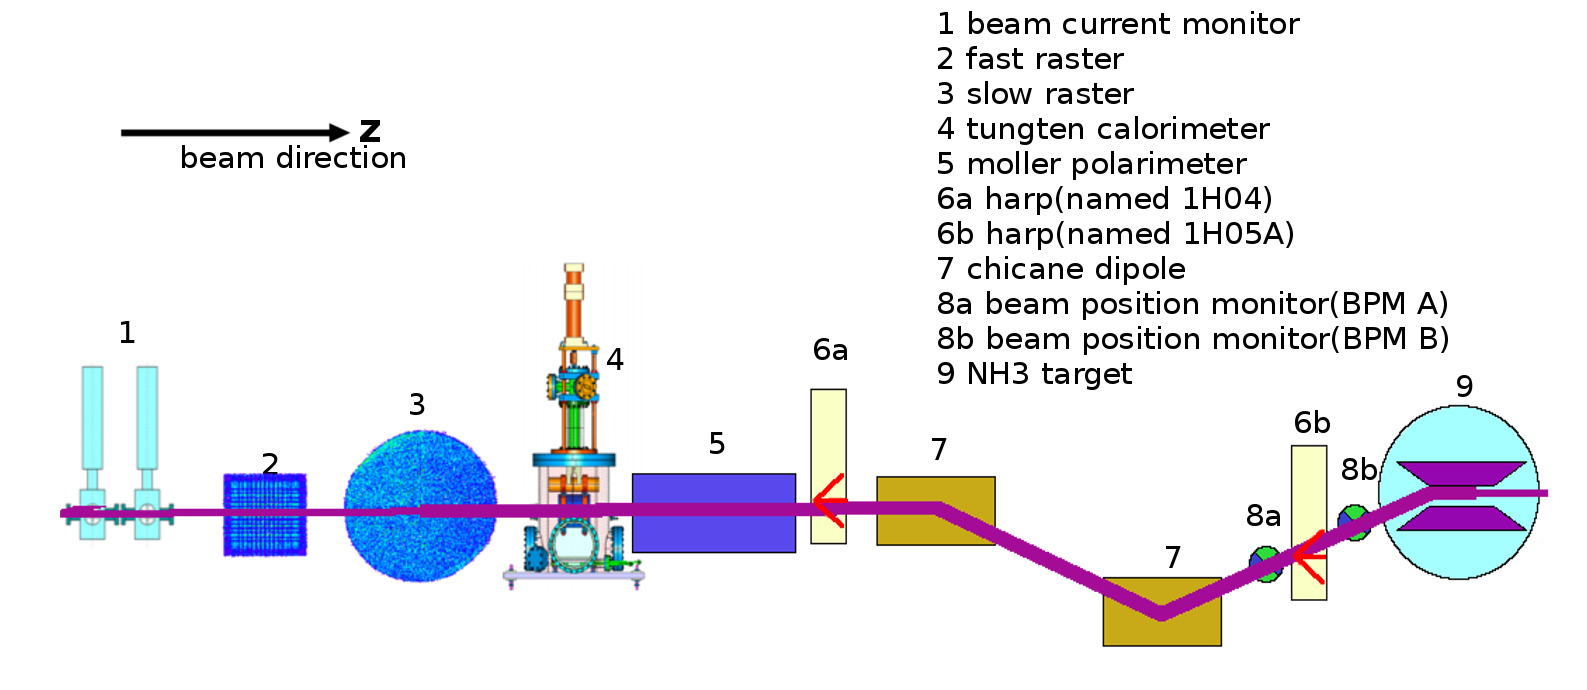
\includegraphics[width=1\linewidth]{beamline_lite} 
\par\end{centering}

\protect\caption{\label{fig:beamline-for-g2p}Schematic of beamline components for
g2p experiment}
\end{figure}



\section{Beam-line Instrumentation}


\subsection{Beam position monitor (BPM)}

The scattering angle of the outgoing lepton in deep inelastic scattering,
which is defined with respect to the direction of the incident beam,
is an important variable for obtaining meaningful physics results.
Therefore, the position and direction of the beam, after being bent
by the chicane magnetic field and spread out by the rasters, must
be measured precisely. Two BPMs and two harps were installed for relative
and absolute measurements of beam position and direction near the
target, respectively.

The BPM consists of four open-ended antennas for detecting the beam
position; the measurement is non-invasive to the beam. The BPM chambers
shown in Fig.\ref{fig:bpm-design-diagram} and Fig. \ref{fig:BPM_daq}
are part of the beam pipe. The four antennas, $x_{+}$, $x_{-}$,
$y_{+}$, $y_{-}$ are attached to feedthroughs on the interior wall
of the pipe at $90^{\circ}$ intervals. 
\begin{figure}[tbph]
\begin{centering}
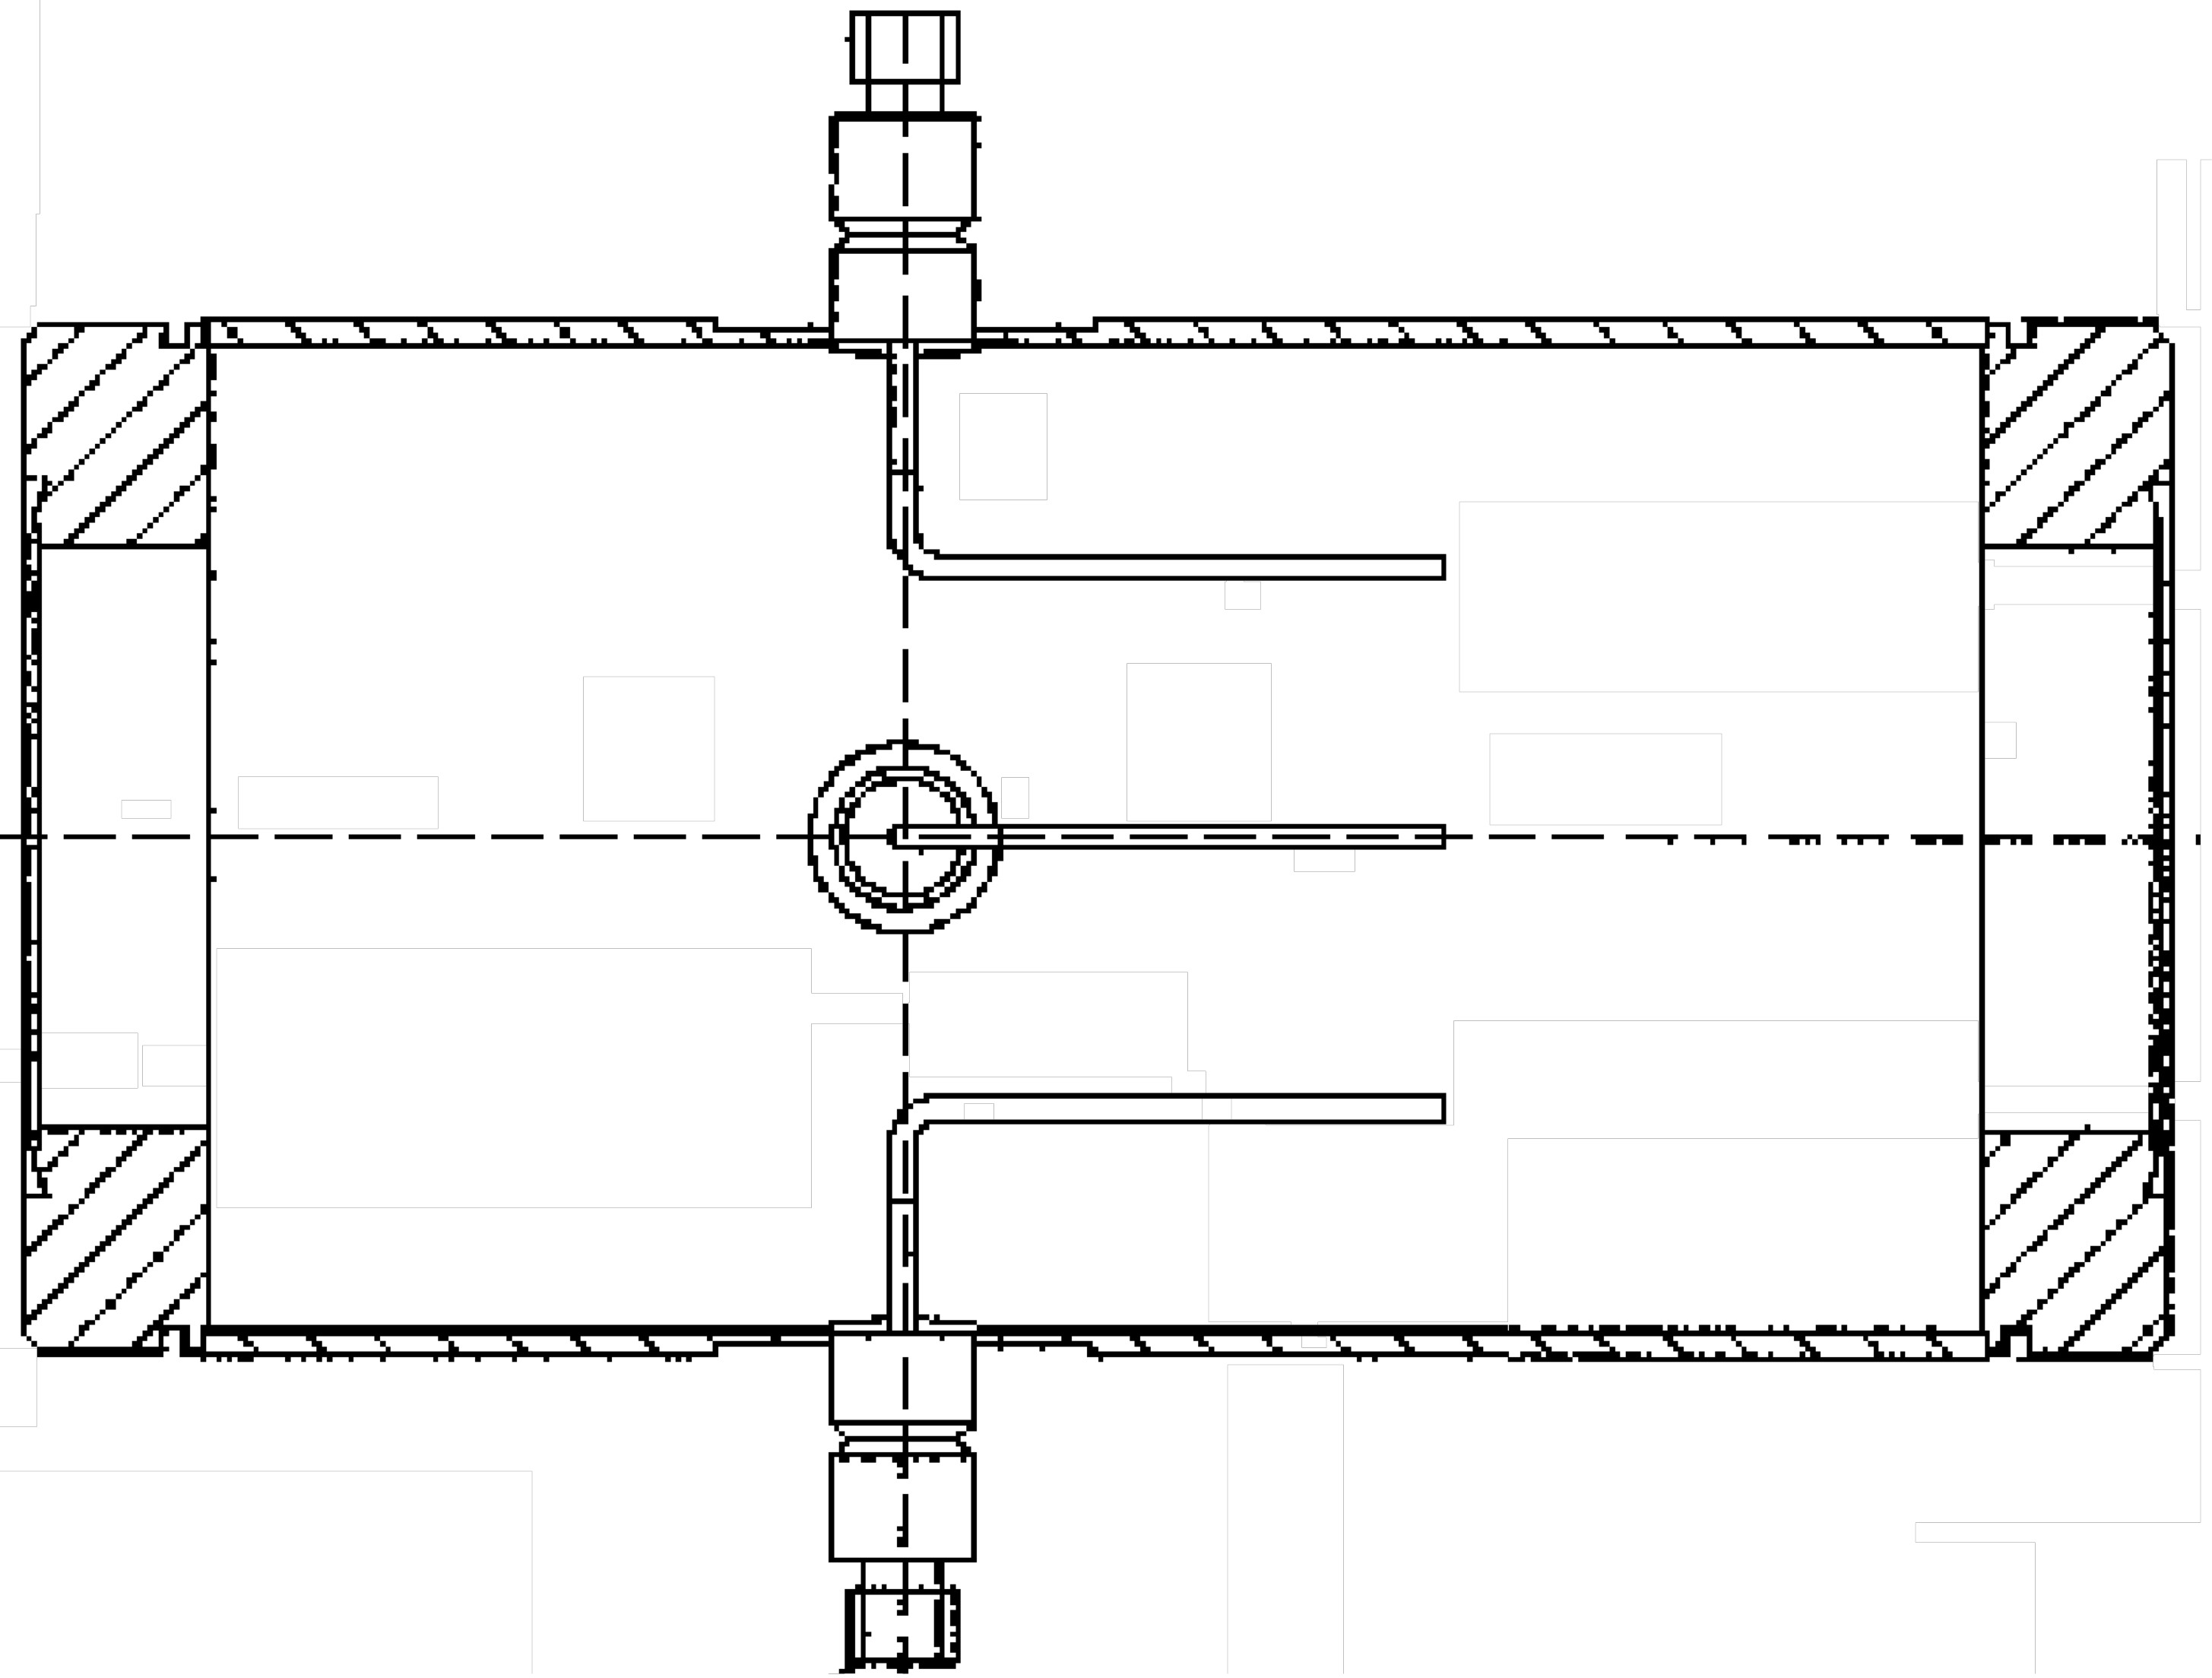
\includegraphics[width=0.4\linewidth]{bpmdiag}
\par\end{centering}

\protect\caption{\label{fig:bpm-design-diagram}BPM chamber design diagram from JLab
instrumentation group}
\end{figure}
\begin{figure}
\begin{centering}
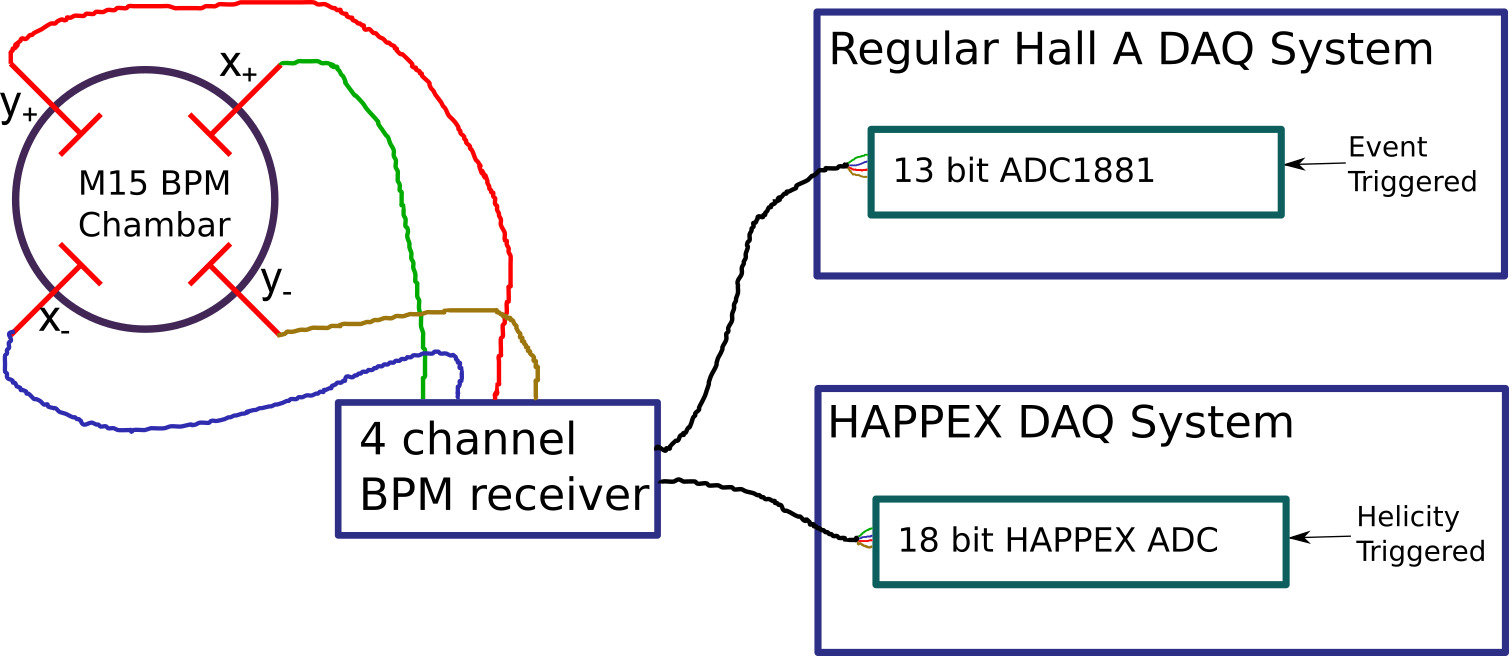
\includegraphics[width=0.7\columnwidth]{bpm_daq}
\par\end{centering}

\protect\caption{\label{fig:BPM_daq}BPM chamber, receiver and related DAQ system for
g2p experiment}
\end{figure}


When the beam passes through the BPM chamber, each antenna receives
an induced signal. As shown in Fig. \ref{fig:BPM_daq}, the BPM receiver
collects and sends the signal to the regular Hall A DAQ system and
another DAQ system designed for parity violation experiments, the
HAPPEX system \citep{ADC18bob}. The new BPM receiver was designed
by the JLab instrumentation group \citep{mussonece652paper} in order
to achieve the required precision at a level of 0.1 mm with a beam
current as low as 50 nA. The regular DAQ system was connected to a
13-bit fastbus ADC (Lecroy ADC 1881) with an integration time of 50
ns, which was triggered by a scattered electron event. The HAPPEX
system was connected to an 18-bit ADC with an integration time of
875 $\mu$s, which was triggered by a beam helicity signal at 1 kHz.
The amplitude, $A$, recorded in the ADC has the following relation
with the BPM signal, $\phi$:

\begin{equation}
A\propto\phi\cdot10^{g/20},\label{eq:adcsignalvsantenna}
\end{equation}
where $g$ is the gain of the receiver.

The BPM receiver generates a large time delay for the output signals.
The digital filter used in the receiver contributes $1/175\,$s delay
time, which was the inverse of the bandwidth setting chosen for the
filter. There is a $\sim4\ \mu$s delay as a result of finite processing
times. The BPM can not provide event by event position because of
this time delay, due to the high frequency fast raster system (discussed
in chapter \ref{sub:Raster-system}).

The existed chicane dipole magnets ordained two BPMs must be installed
after them. Because of the space limitation between the second chicane
magnet and the target, the two BPMs were placed very close to each
other. One was placed 95.5 cm upstream of the target while the other
was placed 69 cm upstream, making the distance between them only 26.5
cm. The short distance magnified the position uncertainty from the
BPMs to target.


\subsection{Super harp}

Two super harps were designed and installed in the beam-line, as shown
in Fig.\ref{fig:beamline-for-g2p} (label 6a - 1H04 and 6b - 1H05A),
to provide an absolute measurement of the beam position for calibration
of the BPMs. The new harps were able to work in pulsed beam (1\% duty
factor) with a current of several $\mu$A. A diagram for the harp
is shown in Fig.\ref{fig:harp-diagram}, 
\begin{figure}[tbph]
\begin{centering}
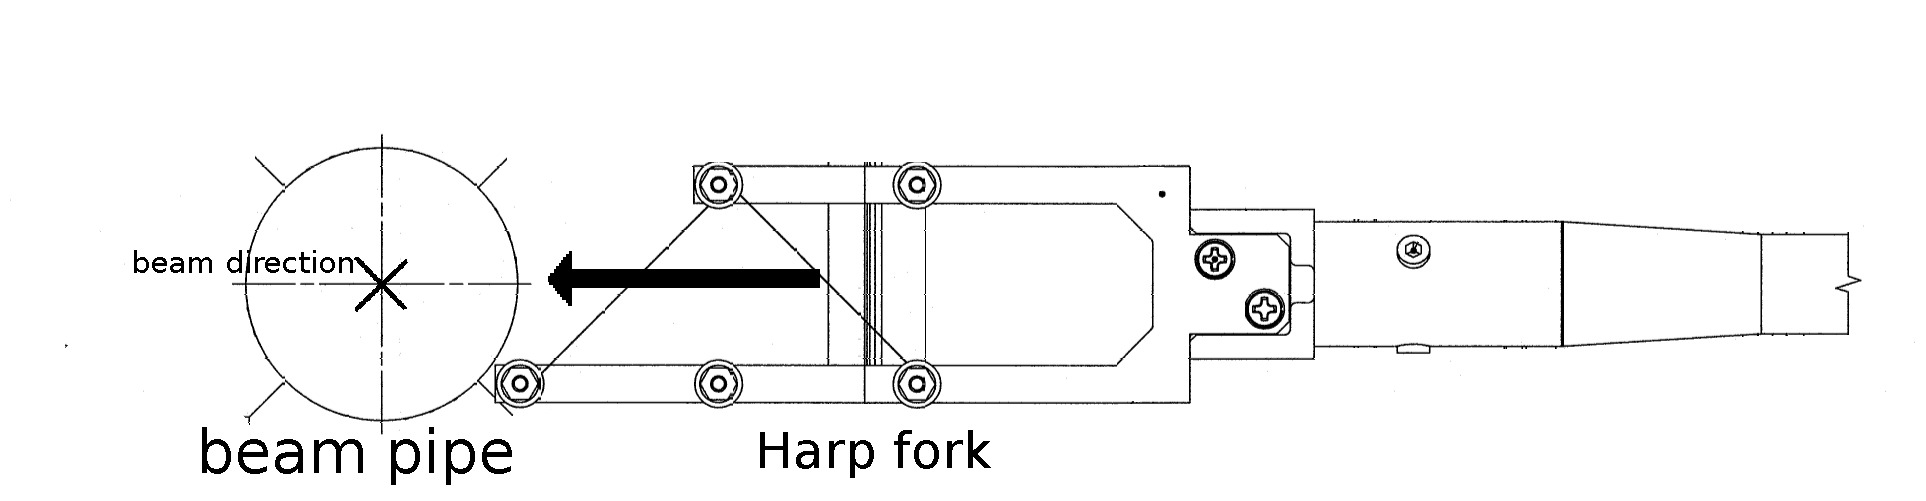
\includegraphics[width=1\linewidth]{harp_one} 
\par\end{centering}

\protect\caption{\label{fig:harp-diagram}Harp diagram}
\end{figure}


which consists of three wires with a thickness of 50 $\mu$m, a fork
and a controller chassis. The harp chamber is perpendicular to the
beam pipe and connected to the beam pipe as part of the vacuum chamber
of the beamline. The two harps have different configurations of three
wires: vertical($|$), bank left($\backslash$), and bank right($/$)
for 1H04, and $/$, $|$, $\backslash$ for 1H05. The angle of the
$/$ or $\backslash$ wires is $45^{\circ}$ relative to the wire
dock frame. The wires are arranged in a fork (Fig.\ref{fig:harp-diagram})
controlled by a step motor \citep{yan261} which can be moved in and
out of the beam-line. The harps must be moved out of the beam-line
when production data is being taken because they are invasive to the
beam. The original position of the wires was surveyed before the experiment
at a precision level of 0.1 mm. As the motor driver moved the fork
through the beam, each wire received a signal, which was recorded
for further analysis. The signals received from the wire and the step-counters
from the motor driver were then sent to an amplifier and the DAQ.
The amplification and the speed of the motor were adjustable for the
purpose of optimizing the signals of each scan. Recorded data combined
with the survey data was used to calculate the absolute beam position.

The signal from the $|$ wire ($peak_{|}$) was used for getting the
$x$ position ($x_{harp}$) of the beam , and the signals from the
$/$, $\backslash$ wires ($peak_{/}$ and $peak_{\backslash}$) were
used for getting the $y$ position ($y_{harp}$): 
\begin{eqnarray}
x_{harp} & = & survey_{|}-peak_{|}\nonumber \\
y_{harp} & = & \frac{1}{2}[(survey_{\backslash}-survey_{/})-(peak_{\backslash}-peak_{/})]\label{eq:harp}
\end{eqnarray}



\subsection{\label{sub:Raster-system}Raster system}

In order to minimize the depolarization, avoid damage to the target
material from radiation, and reduce systematic error for the polarization
measurement by NMR (The polarization of the $NH_{3}$ target was measured
by a NMR coil which installed inside the target cell \citep{Pierce201454}.
The non-uniformity of depolarization could reduce the precision of
the NMR measurement due to the measurement being an average over the
target), two raster systems were installed at $\sim$17 m upstream
of the target, as shown in Fig.\ref{fig:beamline-for-g2p} (labels
2 and 3 for fast and slow rasters, respectively). Both the fast and
slow rasters consist of two dipole magnets. The same triangular waveforms
with frequency of 25 kHz were used to drive the magnet coils of the
fast raster to move the beam in x and y directions, forming a rectangular
pattern of 2 mm$\times$2 mm, as shown in Fig.\ref{fig:Fast-raster}.
\begin{figure}[tbph]
\begin{centering}
\subfloat[Current waveform for the fast raster in x or y channel]{\protect\begin{centering}
\protect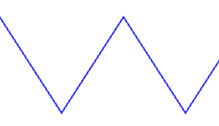
\includegraphics[width=0.25\linewidth]{triangle}\protect
\par\end{centering}

}$\qquad$\subfloat[The 2D histogram of magnet current signals of fast raster]{\protect\begin{centering}
\protect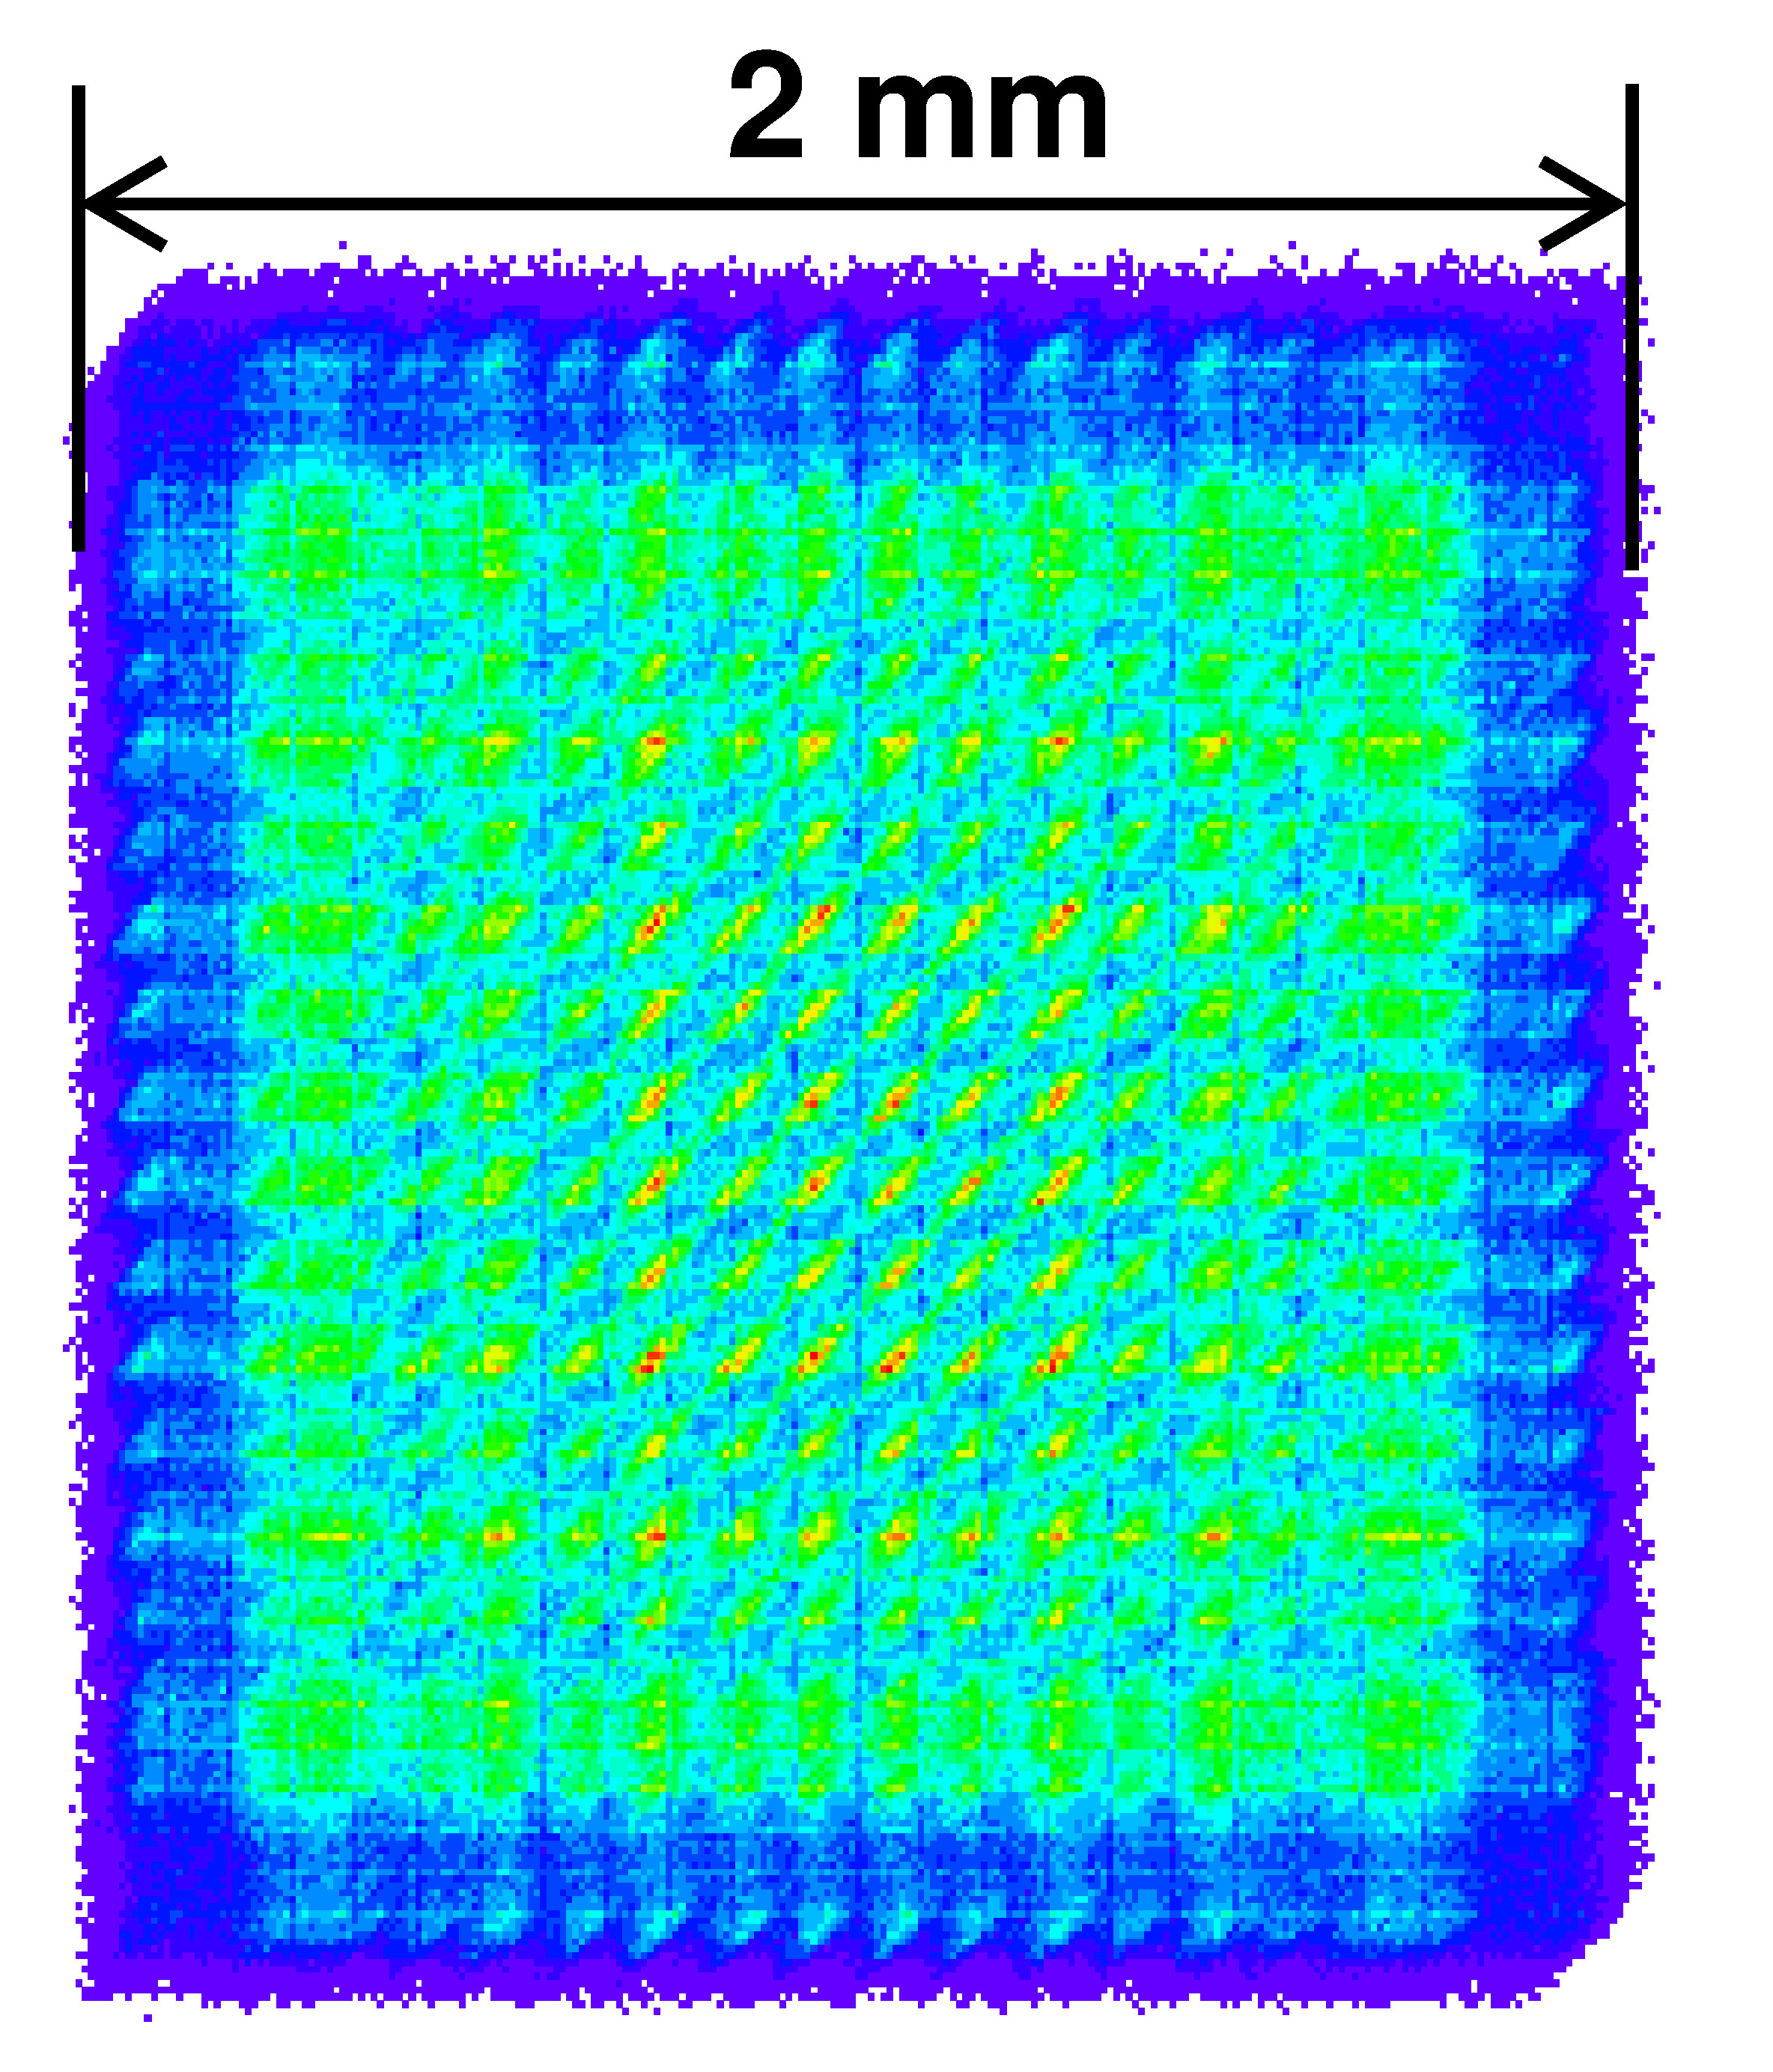
\includegraphics[width=0.2\linewidth]{fast_raster_shape}\protect
\par\end{centering}

}
\par\end{centering}

\protect\caption{\label{fig:Fast-raster}Fast raster pattern}
\end{figure}


A dual-channel function-generator\footnote{agilent 33522A function generator, http://www.home.agilent.com/en/pd-1871286-pn-33522A/function-arbitrary-waveform-generator-30-mhz}
was used to generate two independent waveforms to drive the magnet
coils of the slow raster. 
\begin{figure}[tbph]
\begin{centering}
\subfloat[Current waveform for the slow raster, $t^{\frac{1}{2}}sin(\omega t)$]{\protect\begin{centering}
\protect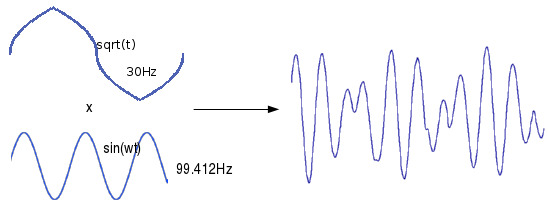
\includegraphics[width=0.7\linewidth]{slow_raster_shape2}\protect
\par\end{centering}

}\subfloat[The 2D histogram of magnet current signals of slow raster]{\protect\begin{centering}
\protect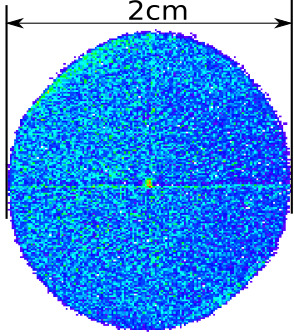
\includegraphics[width=0.2\linewidth]{slow_raster_shape}\protect
\par\end{centering}

}
\par\end{centering}

\protect\caption{\label{fig:Slow-raster}Slow raster pattern }
\end{figure}
 The waveforms for the $x$ and $y$ directions are:

\begin{eqnarray}
x & = & A_{x}(t+amphase_{x})^{1/2}sin(\omega_{x}t+phase_{x}),\nonumber \\
y & = & A_{y}(t+amphase_{y})^{1/2}sin(\omega_{y}t+phase_{y}),\label{eq:slraster_func}
\end{eqnarray}
where the $A_{x}$ and $A_{y}$ are the maximum amplitude, the unit
of $amphase_{x,y}$ is the same as $t$. Both of them are sine functions
modulated by a function $t^{1/2}$ in order to generate a uniform
circular pattern \citep{HCraster200501}, as shown in Fig.\ref{fig:Slow-raster}.
The frequency of the $x$ and $y$ waveforms kept same: $\omega_{x}=\omega_{y}=99.412$
Hz. In order to cycle the amplitude modulation (AM) function, four
piece-wise functions are combined together. The first term is $t^{1/2}$,
and the second term is $period/2-t^{1/2}$, and so on for the third
and fourth terms. The cycled function has the frequency of 30 Hz.
\begin{figure}[tbph]
\begin{centering}
\subfloat[\label{fig:AM-phase-=00003D0022600}AM phase \ensuremath{\neq}0]{\protect\begin{centering}
\protect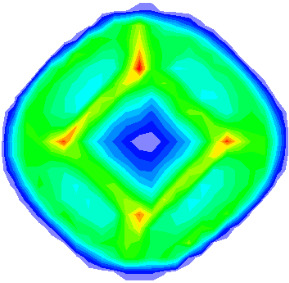
\includegraphics[width=0.33\linewidth]{slraster_uniform_real}\protect
\par\end{centering}

}\subfloat[\label{fig:simulated-raster-shape}simulated raster pattern,with phase=$25^{\circ}$]{\protect\begin{centering}
\protect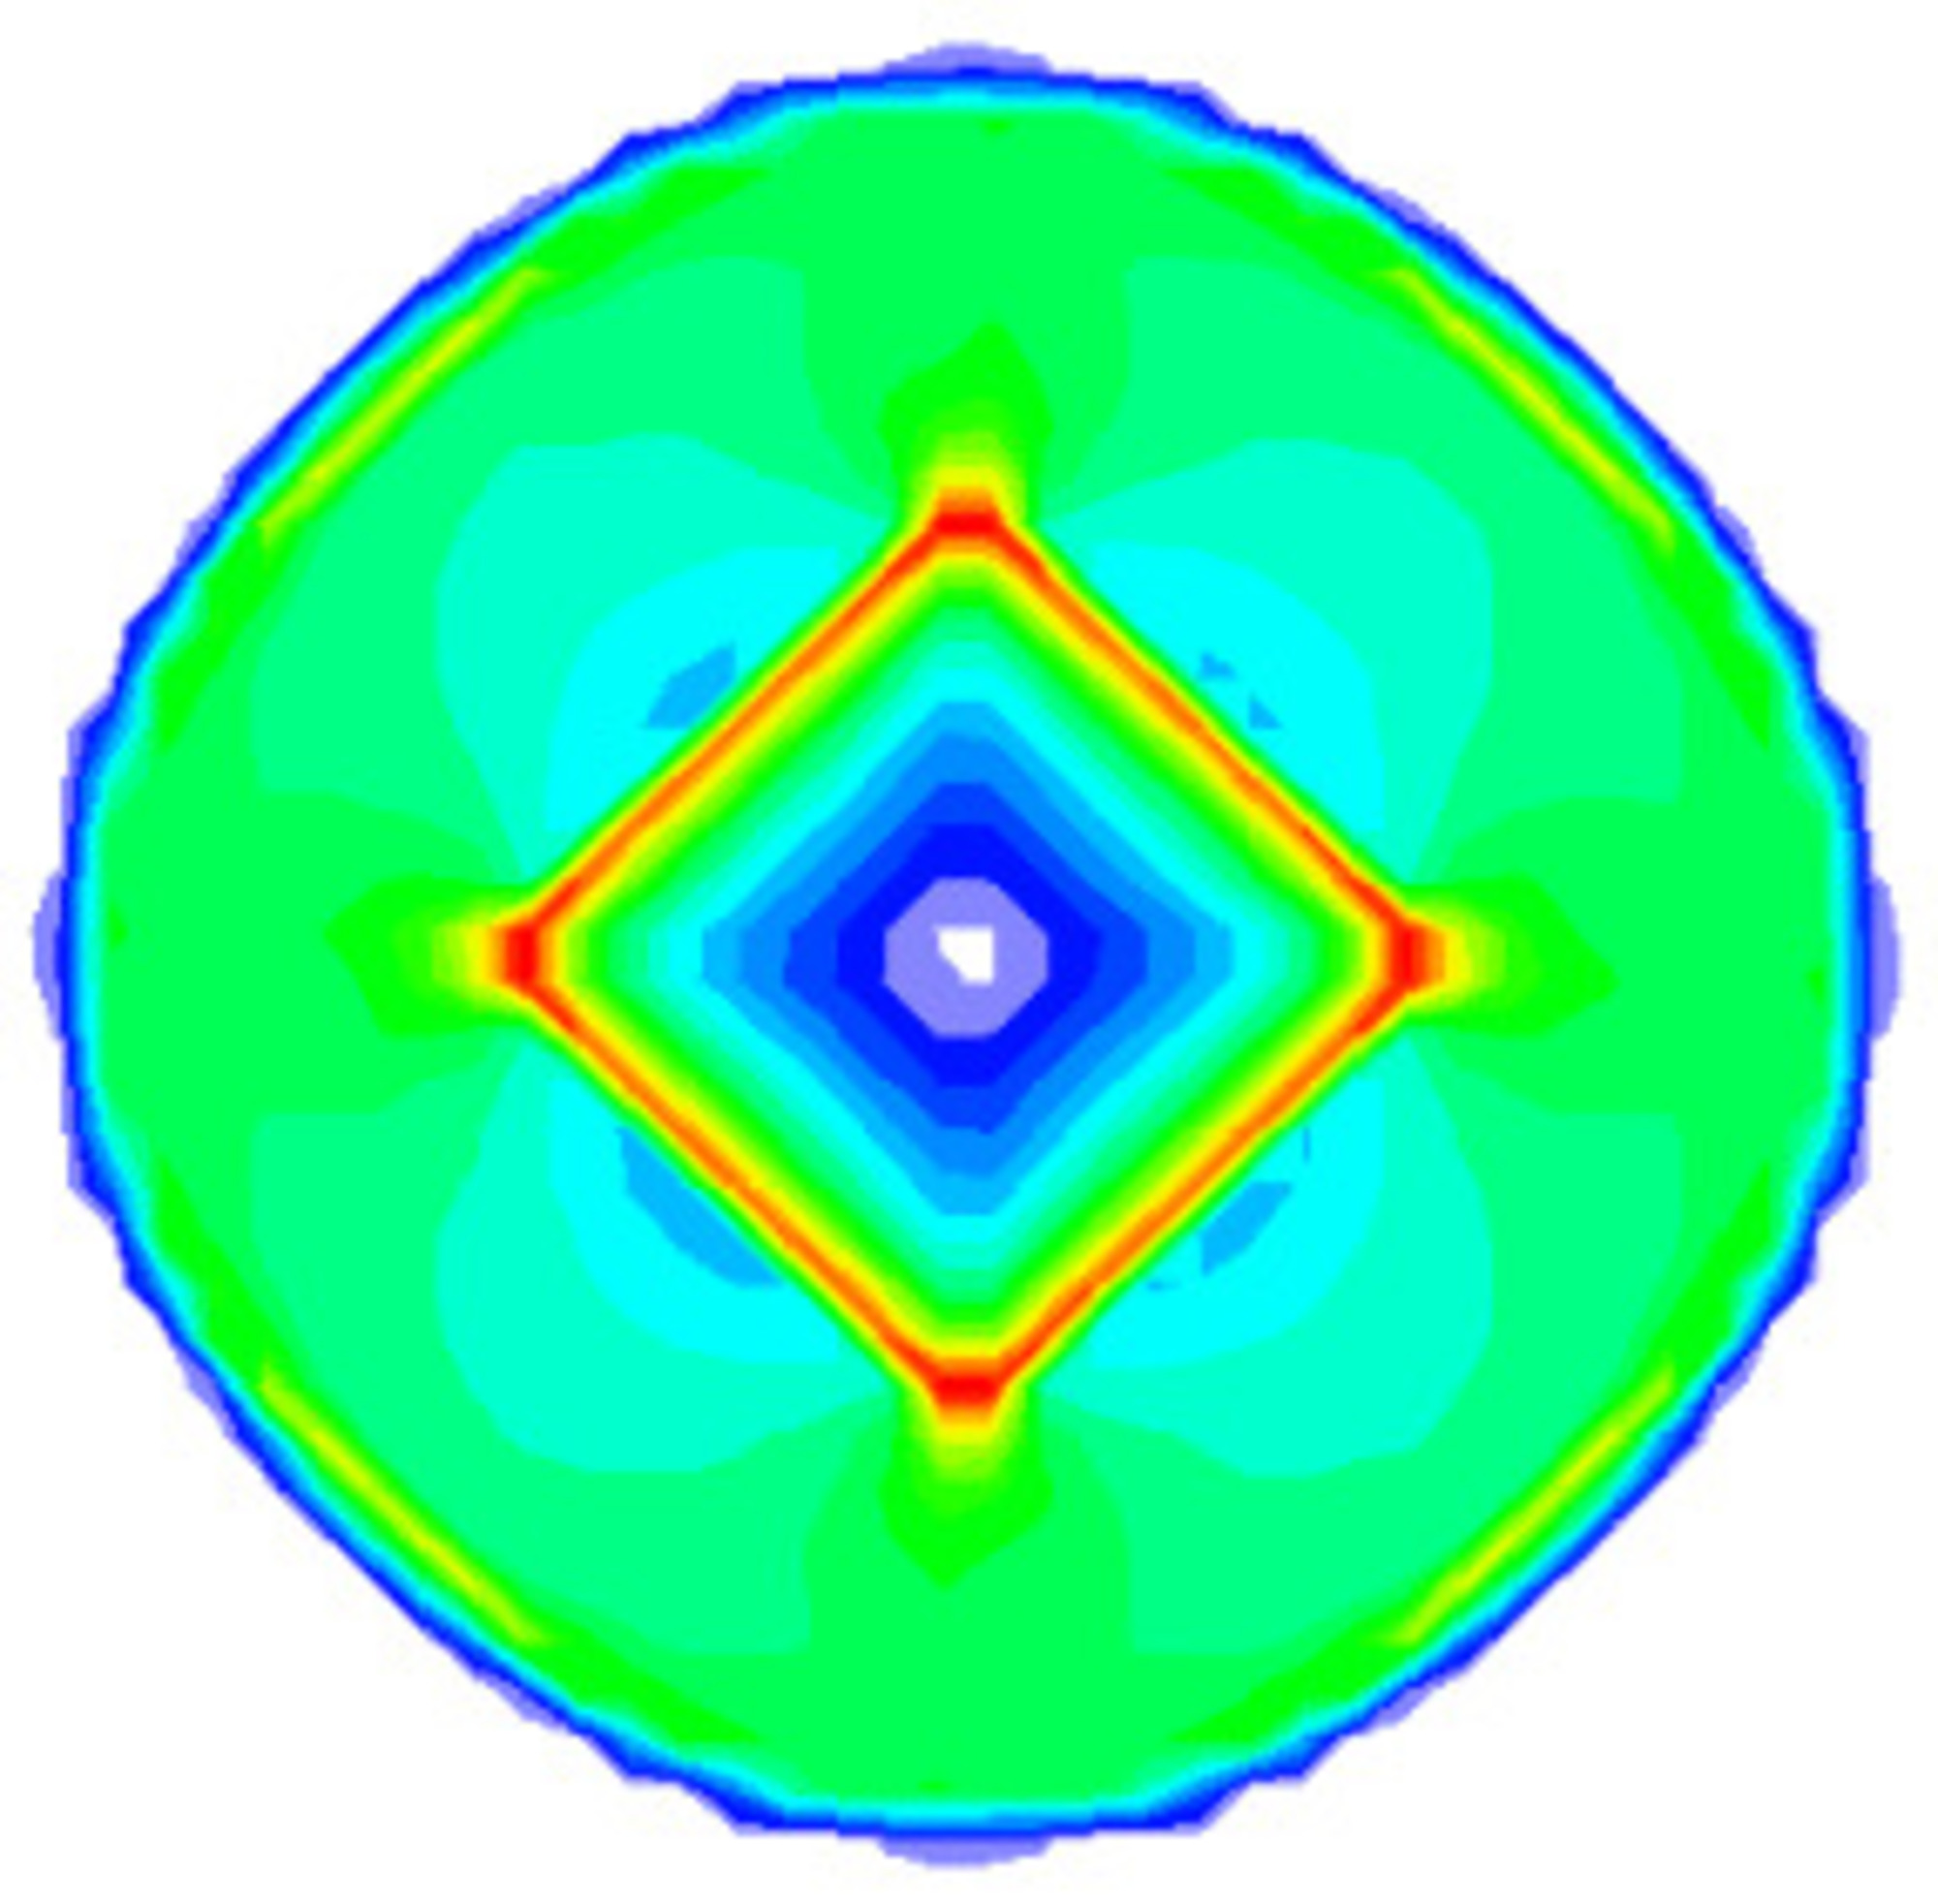
\includegraphics[width=0.33\linewidth]{slraster_uniform_sim}\protect
\par\end{centering}

}\subfloat[\label{fig:AM-phase=00003D00003D0}AM phase=0]{\protect\begin{centering}
\protect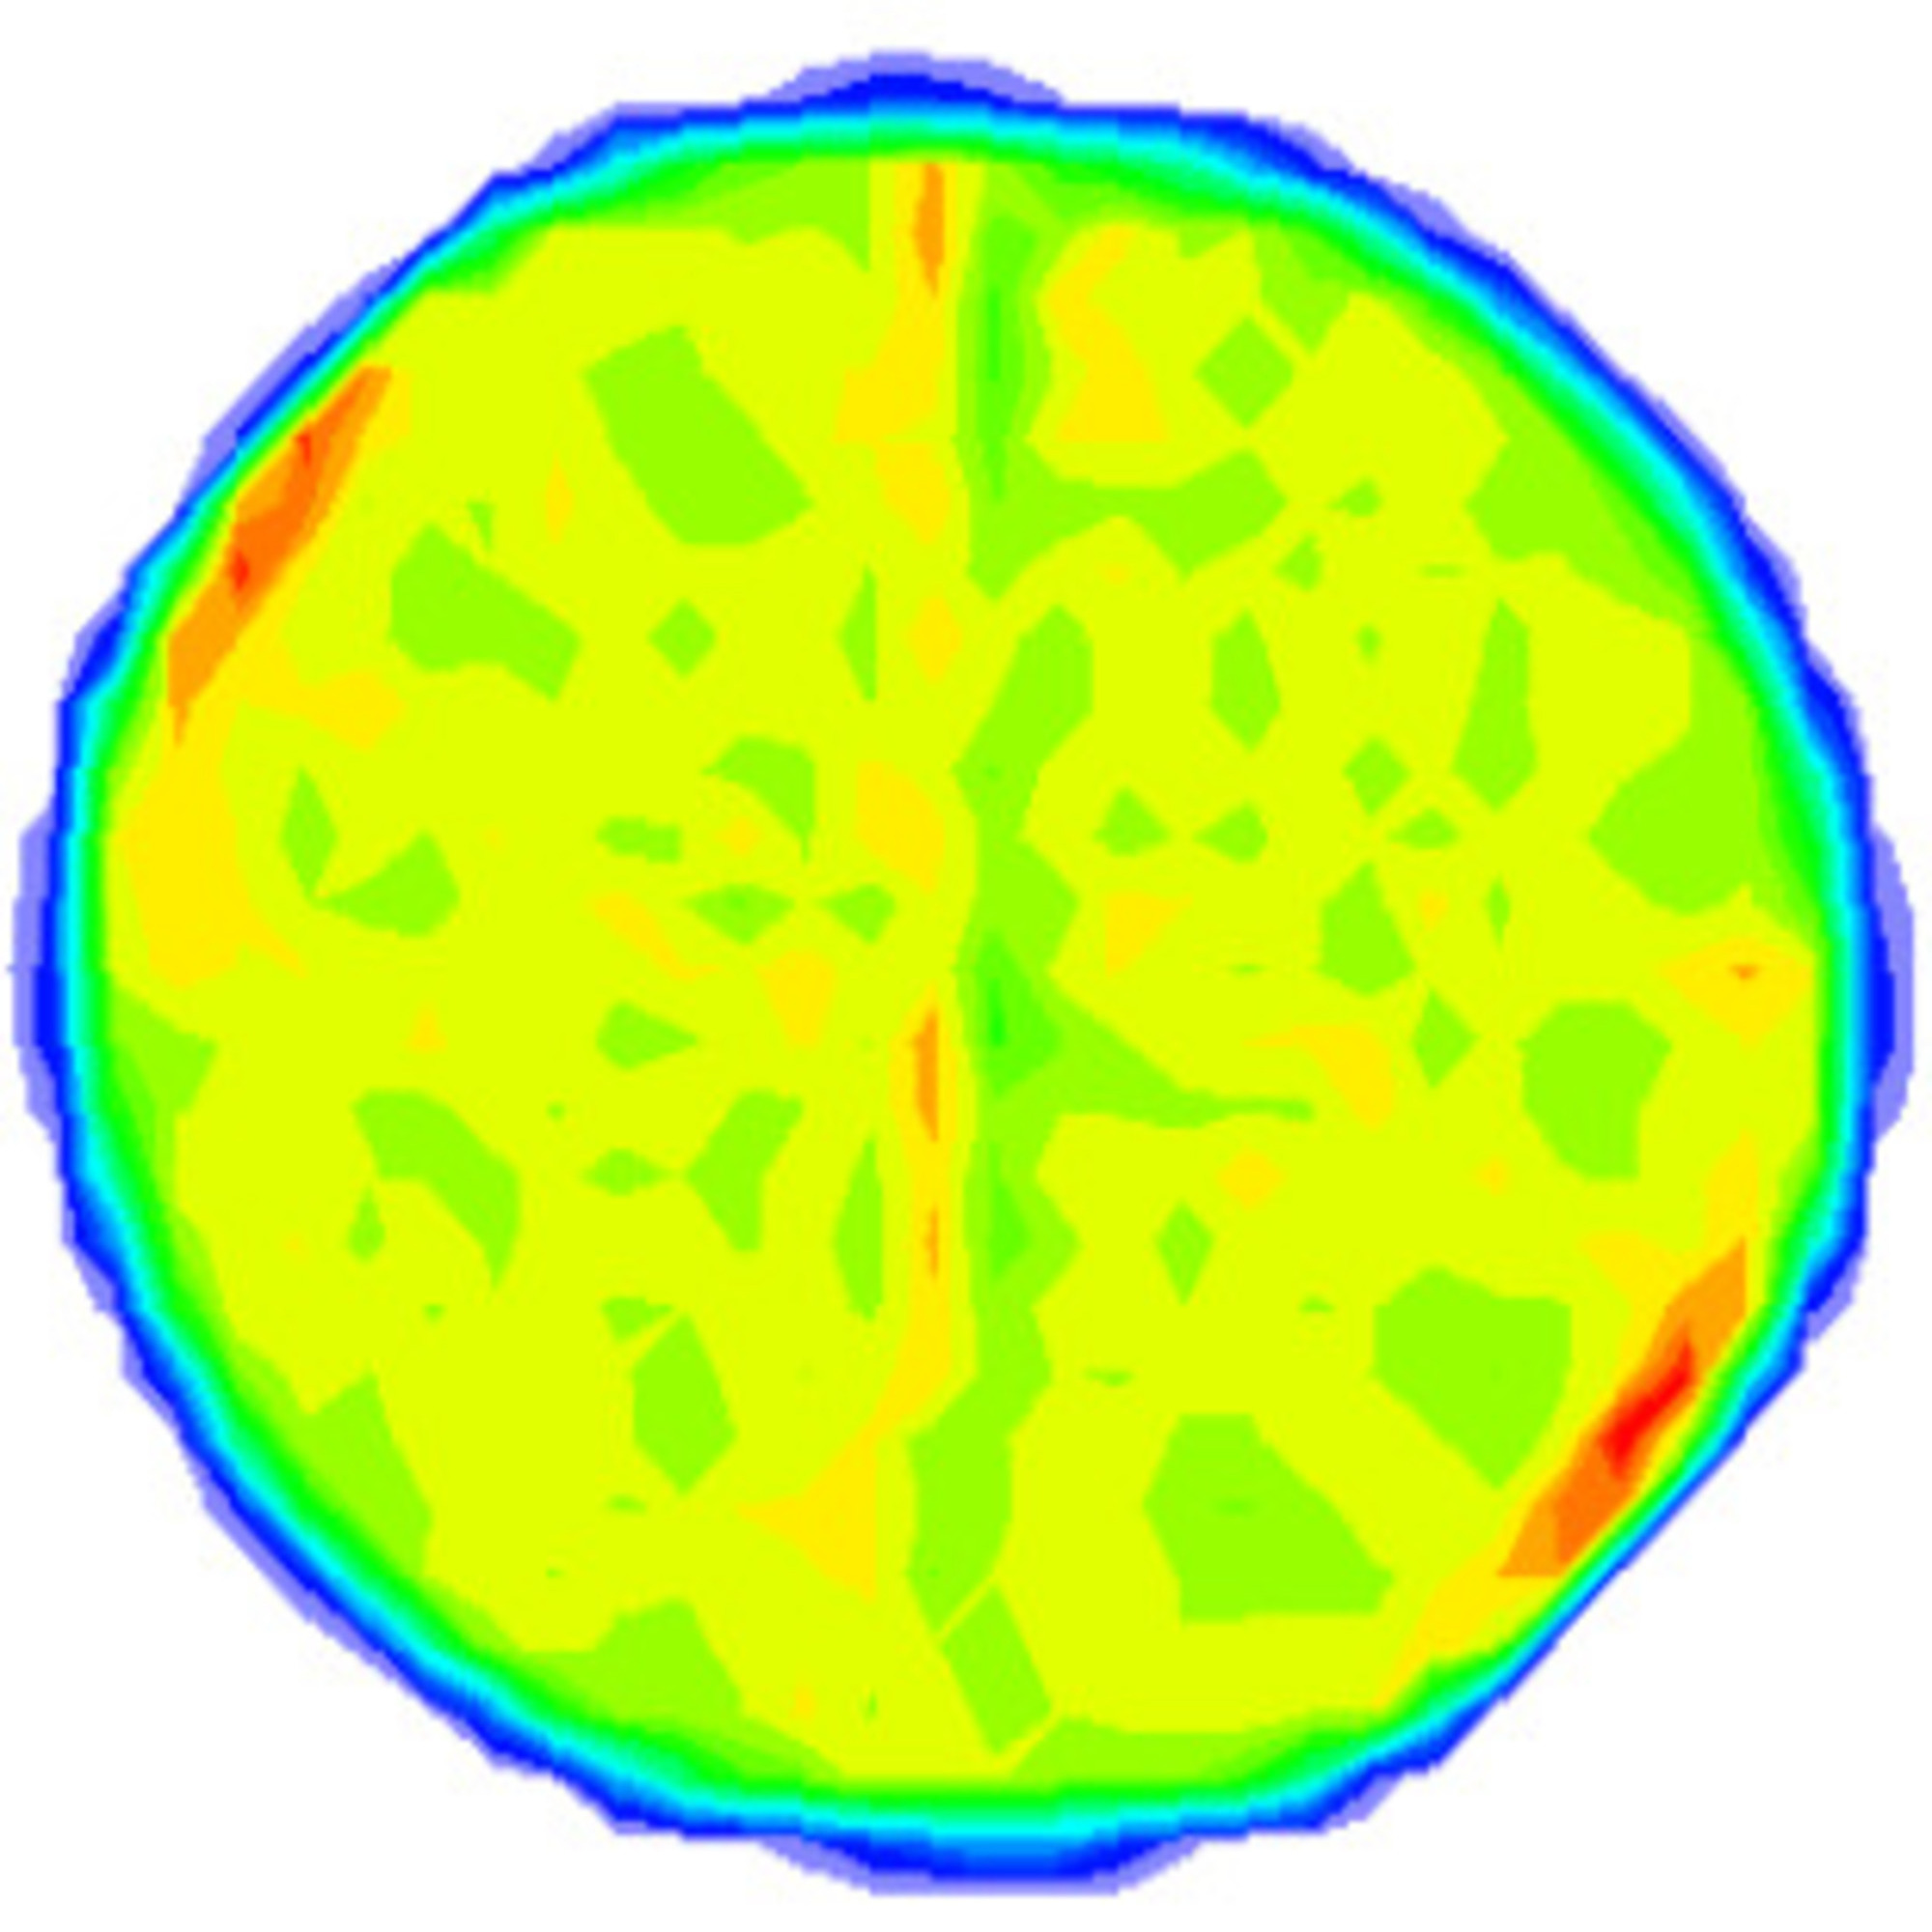
\includegraphics[width=0.33\linewidth]{slraster_uniform}\protect
\par\end{centering}

}
\par\end{centering}

\protect\caption{\label{fig:Slow-raster-uniformity}Slow raster uniformity, (a) and
(c) are from the data, (b) is simulated.}
\end{figure}


Both sine and AM functions have a phase difference between the $x$
and $y$ waveform. The former could be locked by the function generator,
the latter could not be locked and caused a non-uniformity pattern,
as shown in Fig.\ref{fig:Slow-raster-uniformity}(a). A simulation
was done to reproduce the non-uniformity by setting the phase difference
to non-zero, as shown in Fig.\ref{fig:Slow-raster-uniformity}(b).
The phase difference in the AM function was carefully adjusted and
minimized before production data taking to avoid the non-uniformity.
The pattern of the spread beam was relatively uniform after this adjustment
during the experiment, as shown in Fig.\ref{fig:Slow-raster-uniformity}(c).


\section{Data analysis}


\subsection{Coordinate system}

The relationship of coordinate systems used in this paper is shown
in Fig. \ref{fig:Coordinate-systems}.
\begin{figure}
\begin{centering}
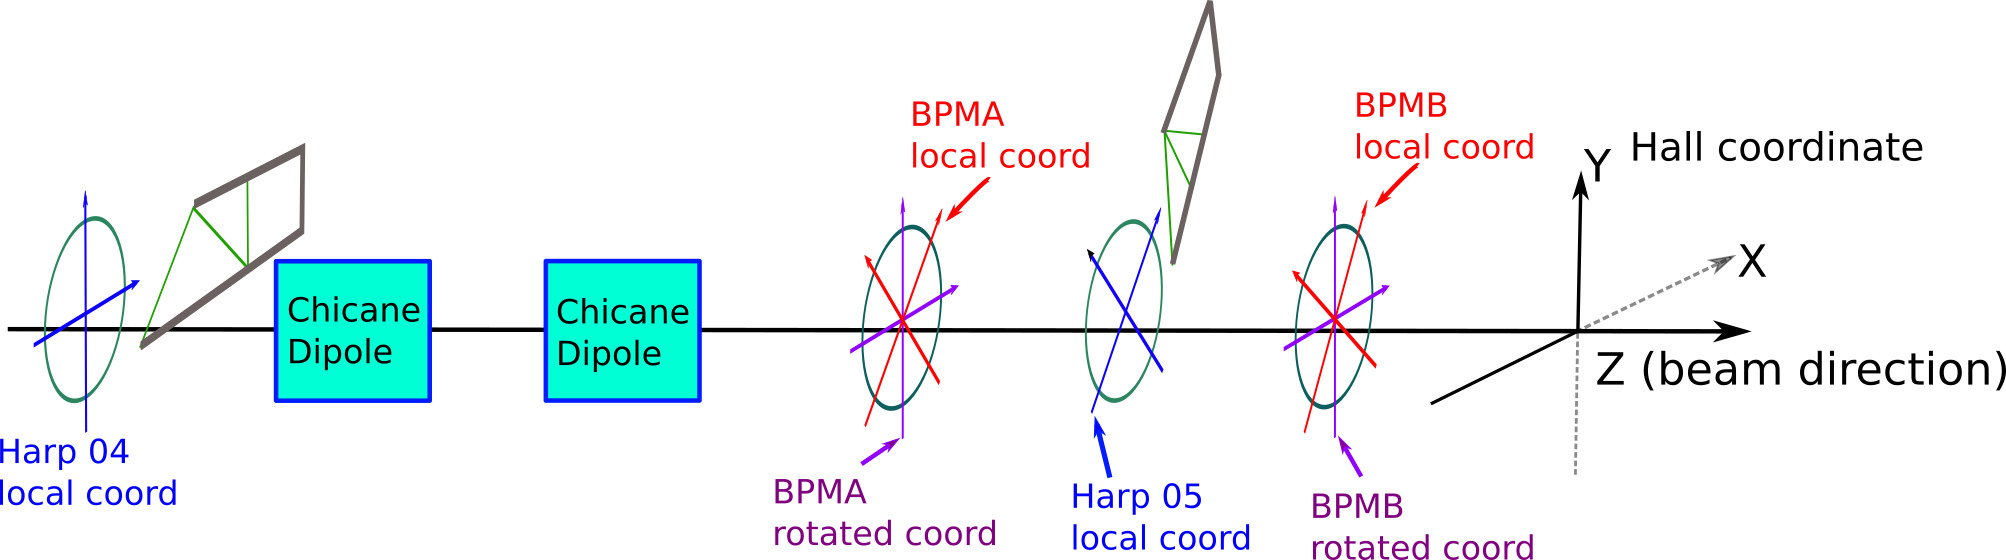
\includegraphics[width=0.95\columnwidth]{bpm_coordinate}
\par\end{centering}

\protect\caption{\label{fig:Coordinate-systems}Coordinate systems used in this paper}
\end{figure}


The Hall coordinate is the global coordinate system in the hall, with
the origin of the $NH_{3}$ target. The positions in the hall coordinate
are identified as capital $X$ and $Y$ .

The origin of each local coordinate system is the surveyed location
for each device. The angular components of survey data decide the
orientation of each local coordinate system. The positions in each
local coordinate system are identified as lowercase $x$ and $y$.
If multi-coordinates are related in the equation, a superscript is
used to indicate the local coordinate system: $x^{bpm/harp}$ and
$y^{bpm/harp}$. The rotation between the BPMA local coordinate and
the Hall coordinate is about $45^{\circ}$, while it is about $57^{\circ}$
between the BPMB local coordinate and the Hall coordinate.

The harp scan data analysis was taken in the harp local coordinate.
The calculated positions from two harps were transferred to the BPM
local coordinate in order to calibrate the BPMs.

The BPM calibration was taken in the BPM local coordinate. In the
straight through setting without the target magnet field, the positions
calculated from the BPMs were transferred to the Hall coordinate in
order to transport to the target location. For the settings with a
transverse magnetic field, the input terms of the transport functions
are the positions in the BPM rotated coordinate, which has the same
origin with the BPM local coordinate but with the same directions
with the Hall coordinate. The positions in the BPM rotated coordinate
are identified as $x^{rot}$ and $y^{rot}$.


\subsection{Harp scans for measuring absolute beam position}

An example of a harp scan result is shown in Fig.\ref{fig:1H05A-harp-scan}.
\begin{figure}[tbph]
\begin{centering}
\subfloat[\label{fig:position-vs-index}position vs index for harp scan, used
for extending position record]{\protect\begin{centering}
\protect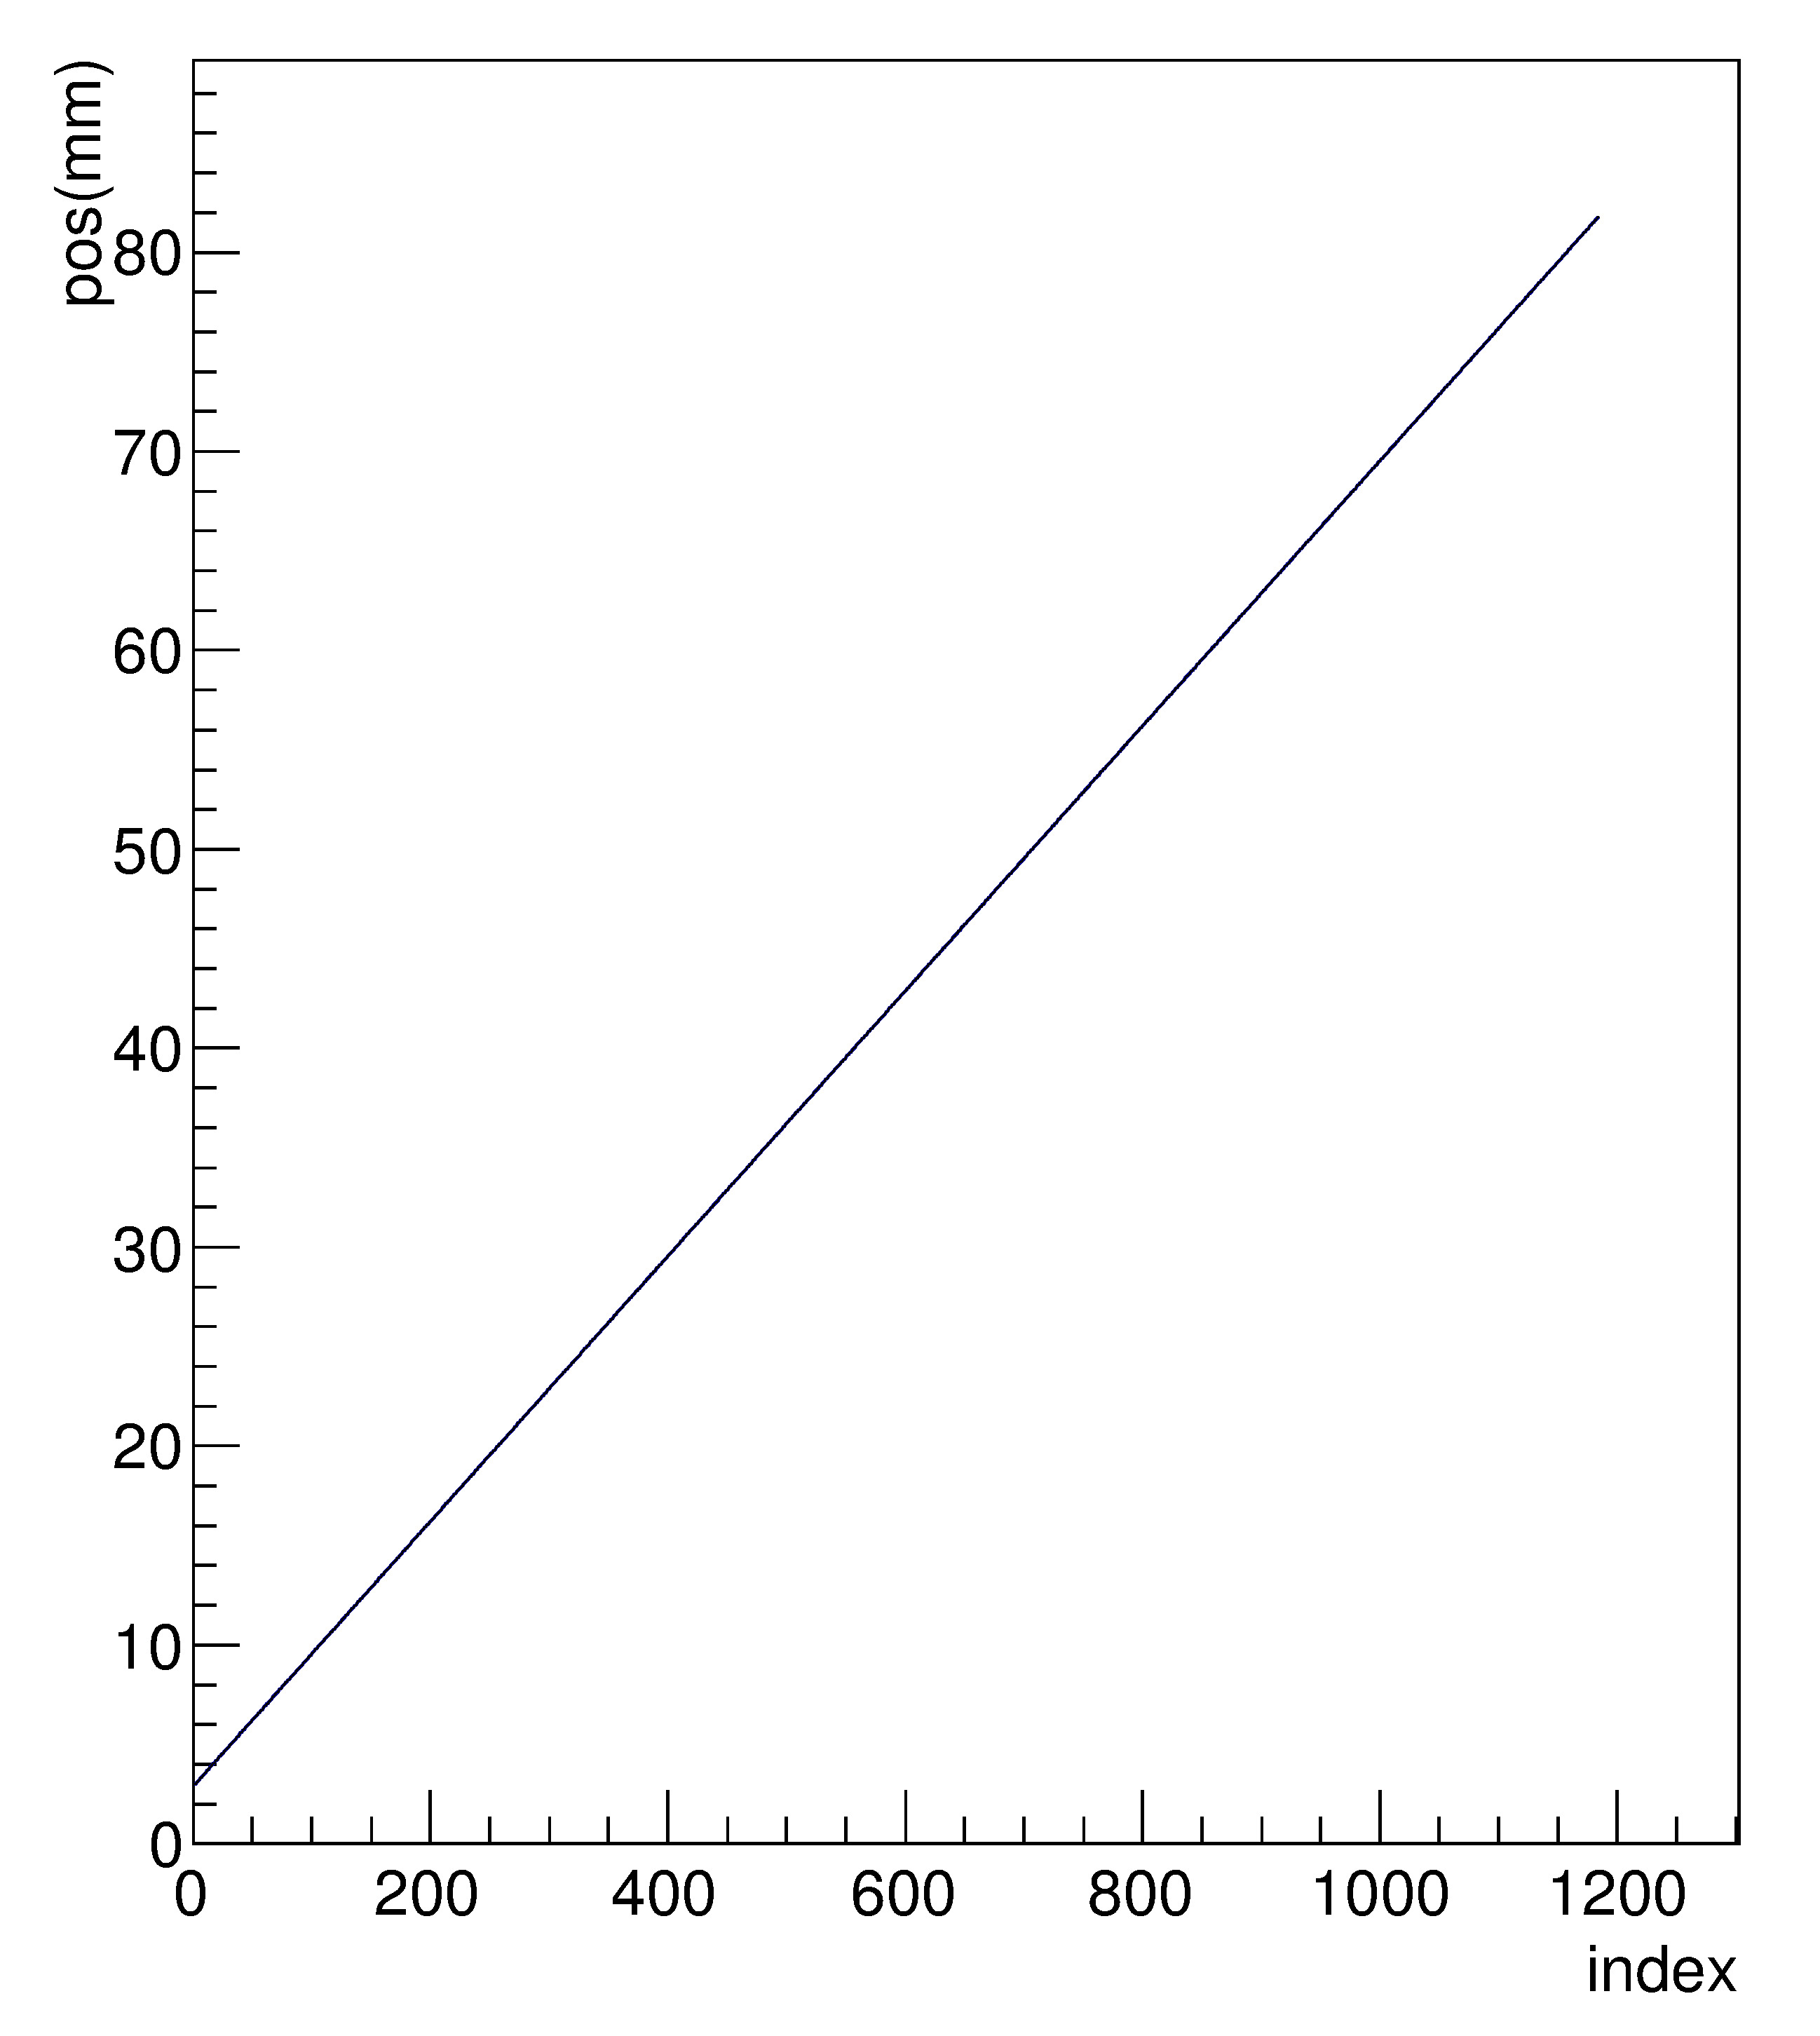
\includegraphics[width=0.4\linewidth]{harp05_pos_index}\protect
\par\end{centering}

}$\qquad$\subfloat[\label{fig:position-vs-signal}Signal vs position for harp, $x$ axis
is position, $y$ axis is the strength of signal. The unit of signal
is the arbitrary ADC unit.]{\protect\begin{centering}
\protect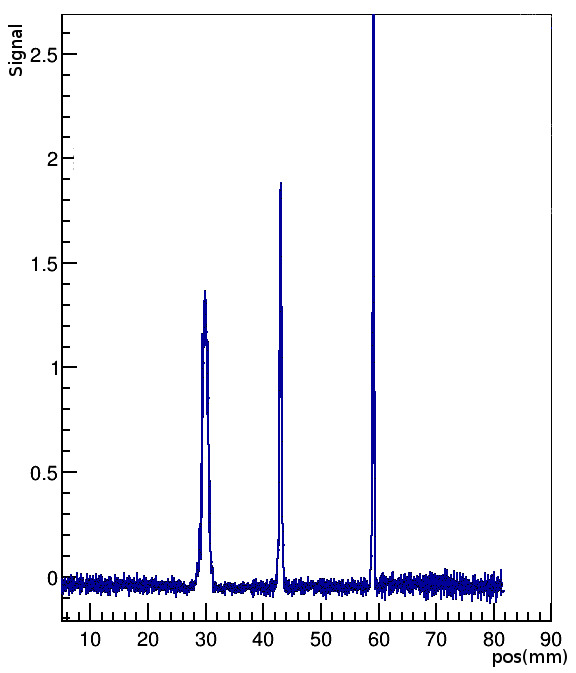
\includegraphics[width=0.4\linewidth]{harp05_peak}\protect
\par\end{centering}

}
\par\end{centering}

\protect\caption{\label{fig:1H05A-harp-scan}1H05A harp scan data}
\end{figure}


There are three groups of recorded data for each harp scan, which
are ``index'', ``position'', and ``signal''. The index is related
to the moving steps of the fork during the scan. Each step of the
index increases by 0.008-0.07 mm depending on the speed of the motor
driver \citep{yan261}. The position is the wire location for each
index. The testing results show a good linear relation between the
position and the index as shown in Fig.\ref{fig:1H05A-harp-scan}(a),
because the motor speed is uniform. The line is the fitted result
with $pos=a*index+b$. According to this linear relation, interpolation
or extrapolation can be applied when a few data points are missing,
in some cases. The strength of signal vs. position is plotted in Fig.\ref{fig:1H05A-harp-scan}(b).
Each peak represents the location when one of the three wires passed
through the beam.

The positions measured by the two harps were used for calibrating
the beam positions in the two BPMs. When the chicane magnets were
on, beam did not pass straight through from the first harp to the
second harp. BPM calibrations using two harps were only possible when
the chicane magnets were off, i.e. in the straight-through settings.
Since the BPM was calibrated in the local coordinate system, the calibration
constants were independent from the settings of other instruments.
To make sure that the calibration constants for the BPMs were still
valid during the non-straight-through settings, the settings for the
BPM receiver were kept the same as in the straight-through settings
during production running.

The scan data from the harps was not reliable when the current of
CW beam (100\% duty factor) was lower than 100 nA due to the low signal-to-noise
ratio. The harp scans were taken in pulsed mode at a current of a
few $\mu$A, while the BPMs were used for production data taking in
CW mode at a beam current of 50-100 nA. For a BPM calibration run,
a harp scan was done first in pulsed mode, then a DAQ run was taken
immediately to record the ADC value in CW mode without changing the
beam position. The harp scan was then taken again in the pulsed mode
to double check the beam position. The harp scan data was discarded
and the scan was taken again if the beam position changed.


\subsection{BPM data analysis and calibration}

The traditional diff/sum method to calculate the beam position has
the non-linearity effect in the position far away from the center
of the beam pipe \citep{Barry301}. It is necessary to correct the
equation of diff/sum since we have a slow raster. From the method
of image \citep{carmanbpm,piotbpm}, the signal from each antenna
excited by the beam can be calculated by: 

\begin{equation}
\phi_{i}=\phi_{0}I\frac{R^{2}-\rho^{2}}{R^{2}+\rho^{2}-2R\rho cos(\theta_{i}-\theta_{0})},\label{eq:antenna_signal}
\end{equation}
where $\phi_{i}$ is the signal received in the antenna, and $i$
is $x_{+}$, $x_{-}$, $y_{+}$ and $y_{-}$, respectively, $\phi_{0}$
is a constant related to the geometry of the BPM-chamber and the output
resistance, $I$ is the beam current, $R$ is the radius of the BPM
vacuum chamber, $\rho$ is the radial position of the beam, and $\theta_{i}-\theta_{0}$
is the angle difference between the antenna and the beam in the polar
coordinate . 
\begin{figure}[tbph]
\begin{centering}
\subfloat[Mirror method]{\protect\begin{centering}
\protect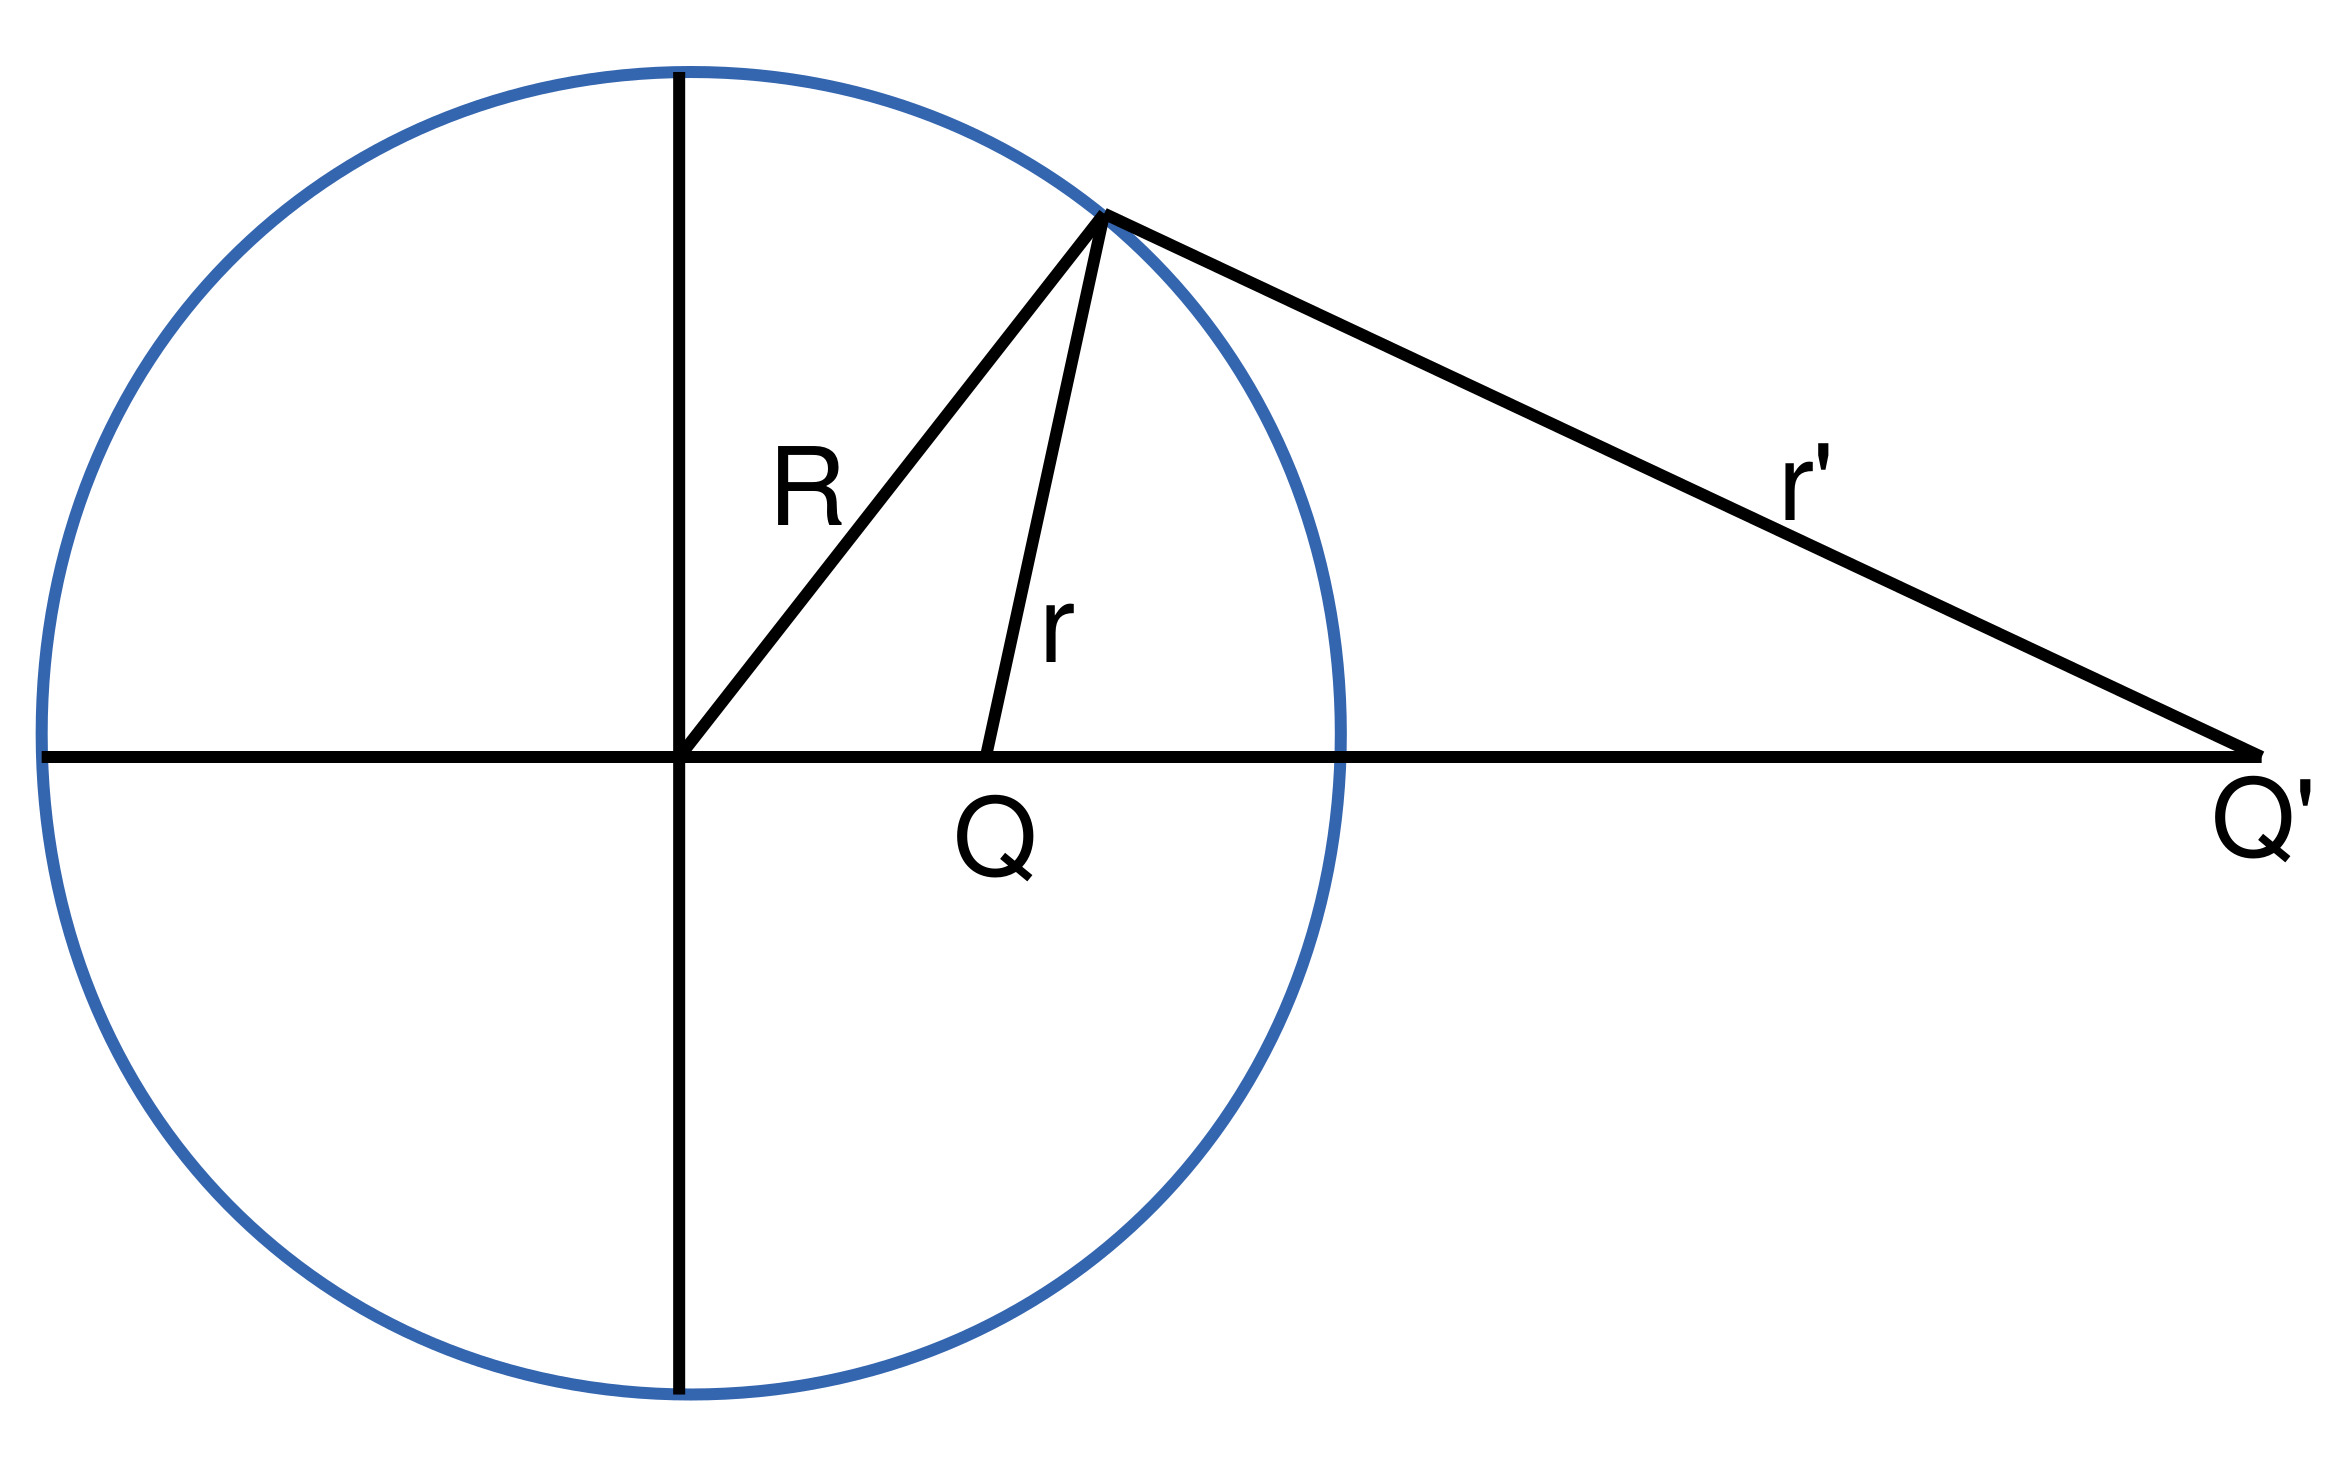
\includegraphics[width=0.4\linewidth]{mirror_method}\protect
\par\end{centering}

}\subfloat[Signal on antenna]{\protect\begin{centering}
\protect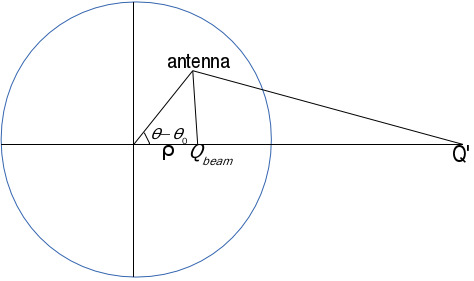
\includegraphics[width=0.4\linewidth]{antenna_signal}\protect
\par\end{centering}

}
\par\end{centering}

\protect\caption{\label{fig:mirror_method}Signal for each antenna of BPM}
\end{figure}


The four antennas in the BPM chamber are used to determine the beam
positions $x$ and $y$ in the BPM; $x_{+}$ and $x_{-}$ for the
$x$ position, and $y_{+}$ and $y_{-}$ for the $y$ position. In
order to extract the beam position information, and eliminate the
dependence on the beam current in equation (\ref{eq:antenna_signal}),
the difference-over-sum method is used as follows:

\begin{eqnarray}
x_{d} & = & \frac{\phi_{x+}-\phi_{x-}}{\phi_{x+}+\phi_{x-}},\label{eq:diff/sum}\\
y_{d} & = & \frac{\phi_{y+}-\phi_{y-}}{\phi_{y+}+\phi_{y-}}.\label{eq:diff/sumy}
\end{eqnarray}
Substituting equation (\ref{eq:antenna_signal}) into equation (\ref{eq:diff/sum})
and equation (\ref{eq:diff/sumy}), they can be rewritten as follows:

\begin{equation}
x_{d}=\frac{\phi_{x+}-\phi_{x-}}{\phi_{x+}+\phi_{x-}}=\frac{2}{R}\frac{\rho cos(\theta-\theta_{0})}{1+\frac{\rho^{2}}{R^{2}}}=\frac{2}{R}\frac{x}{1+\frac{x^{2}+y^{2}}{R^{2}}},\label{eq:xb=00003D000026xy}
\end{equation}


\begin{equation}
y_{d}=\frac{2}{R}\frac{y}{1+\frac{x^{2}+y^{2}}{R^{2}}},\label{eq:yb=00003D000026xy}
\end{equation}
where $\rho^{2}=x^{2}+y^{2}$. When $x^{2}+y^{2}\ll R^{2}$, equations
(\ref{eq:xb=00003D000026xy}) and (\ref{eq:yb=00003D000026xy}) can
be simplified as:

\begin{eqnarray}
x & = & \frac{R}{2}x_{d}=\frac{R}{2}\frac{\phi_{x+}-\phi_{x-}}{\phi_{x+}+\phi_{x-}},\nonumber \\
y & = & \frac{R}{2}y_{d}=\frac{R}{2}\frac{\phi_{y+}-\phi_{y-}}{\phi_{y+}+\phi_{y-}}.\label{eq:litexyb=00003D000026xy}
\end{eqnarray}
Equation (\ref{eq:litexyb=00003D000026xy}) can be used in the simple
case when the beam is near the center of the beam pipe. When the beam
is far from the center, equation (\ref{eq:litexyb=00003D000026xy})
is no longer valid. For the g2p experiment, the beam was rastered
to have a diameter of about 2 cm at the target. Combining equation
(\ref{eq:xb=00003D000026xy}) with (\ref{eq:yb=00003D000026xy}) the
beam position can be calculated as:

\begin{eqnarray}
x & = & Rx_{d}(\frac{1}{x_{d}^{2}+y_{d}^{2}}-\frac{1}{\sqrt{x_{d}^{2}+y_{d}^{2}}}\sqrt{\frac{1}{x_{d}^{2}+y_{d}^{2}}-1}),\nonumber \\
y & = & Ry_{d}(\frac{1}{x_{d}^{2}+y_{d}^{2}}-\frac{1}{\sqrt{x_{d}^{2}+y_{d}^{2}}}\sqrt{\frac{1}{x_{d}^{2}+y_{d}^{2}}-1}).\label{eq:realxy}
\end{eqnarray}
To verify this corrected equation, a simulation was performed. First,
a set of position data was generated (Fig.\ref{fig:Simulated-real-position}(a)),
\begin{figure}[tbph]
\begin{centering}
\subfloat[\label{fig:diff_sum_simulated}]{\protect\begin{centering}
\protect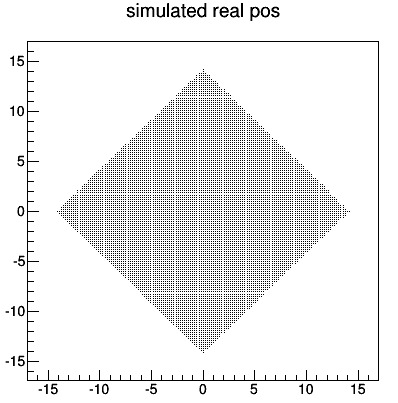
\includegraphics[width=0.3\linewidth]{diff_sum_simreal}\protect
\par\end{centering}

}\subfloat[\label{fig:diff_sum_calculated}]{\protect\begin{centering}
\protect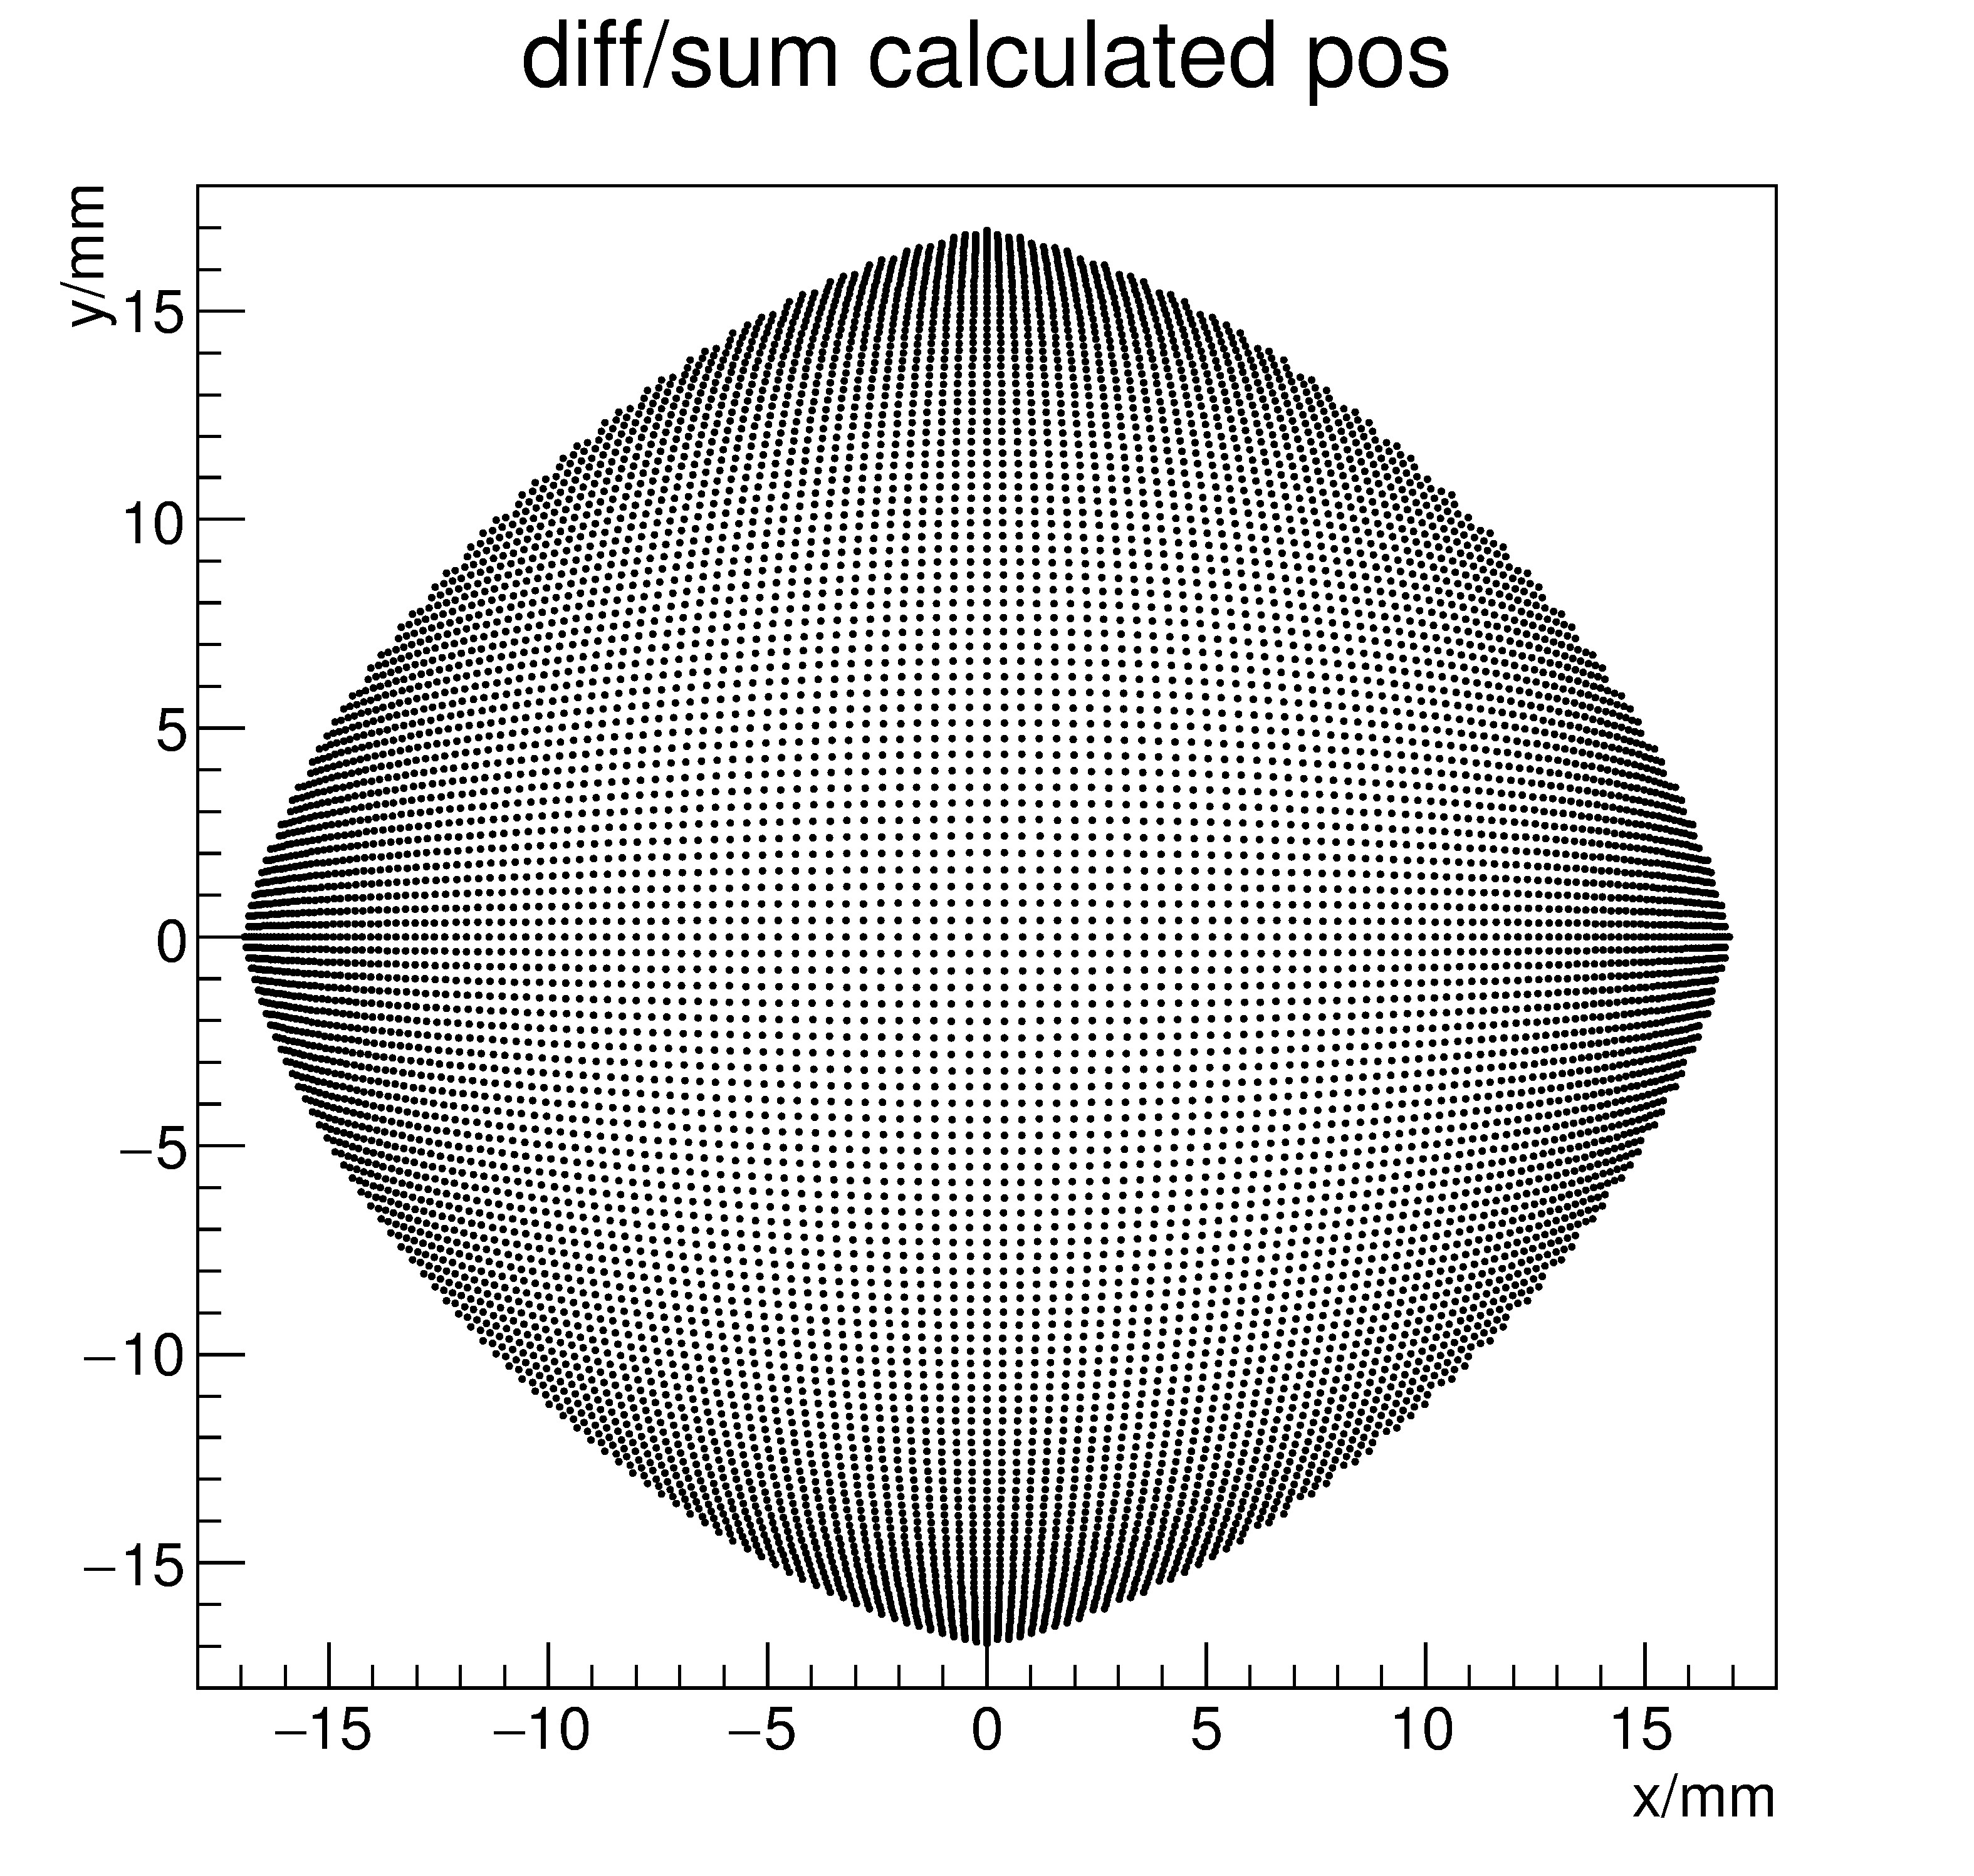
\includegraphics[width=0.3\linewidth]{diff_sum_calculated}\protect
\par\end{centering}

}\subfloat[\label{fig:diff_sum_correction}]{\protect\begin{centering}
\protect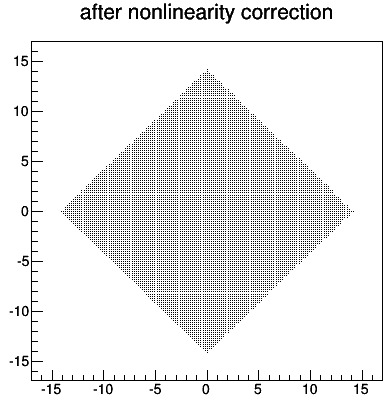
\includegraphics[width=0.3\linewidth]{diff_sum_correction}\protect
\par\end{centering}

}
\par\end{centering}

\protect\caption{\label{fig:Simulated-real-position}Comparing the calculated results
using equation (\ref{eq:litexyb=00003D000026xy}) and (\ref{eq:realxy})
with simulated position. (a) Simulated position; (b) The calculated
result with equation (\ref{eq:litexyb=00003D000026xy}), (c) The calculated
result with equation (\ref{eq:realxy}).}
\end{figure}
and the designed radius for the BPM chamber was used for $R$. Using
equation (\ref{eq:antenna_signal}) to get the signal for each antenna,
and setting $\phi_{0}$ and $I$ to be equal to 1, equations (\ref{eq:litexyb=00003D000026xy})
and (\ref{eq:realxy}) were used to calculate the beam position. The
results are shown in Fig.\ref{fig:Simulated-real-position}(b) and
\ref{fig:Simulated-real-position}(c), respectively. In this way the
method using equation (\ref{eq:realxy}) can correct the non-linearity
effect caused by equation (\ref{eq:litexyb=00003D000026xy}). Assuming
the slow raster spreads the beam uniformly by changing the slow raster
magnet current, the slow raster magnet current can be used to check
this non-linearity. The slow raster magnet current can be converted
to the displaced position, more details about the conversion will
be discussed in chapter \ref{sub:Det-ebe-pos}. Fig. \ref{fig:Linearityraster}
shows the linearity of the corrected equation with the position converted
from the slow raster, compared with position calculated from the diff/sum
equation. In order to avoid the delay time caused by the BPM receiver,
the waveform of the slow raster x-magnet was set to 20 Hz sinusoidal
for this study. The slow raster y-magnet and the fast raster were
kept off. Since the BPM has a $45^{\circ}$ rotation with the Hall
coordinate, the beam was sweeping in the diagonal direction in the
BPM local coordinate, which has the largest non-linearity effect from
the Fig. \ref{fig:Simulated-real-position}(c). The result shows that
the corrected equation has a better linearity than the diff/sum one.
Better solution may use a corrected algorithm during the benchmark
test of the hardware \citep{p.TUPC172}.
\begin{figure}
\begin{centering}
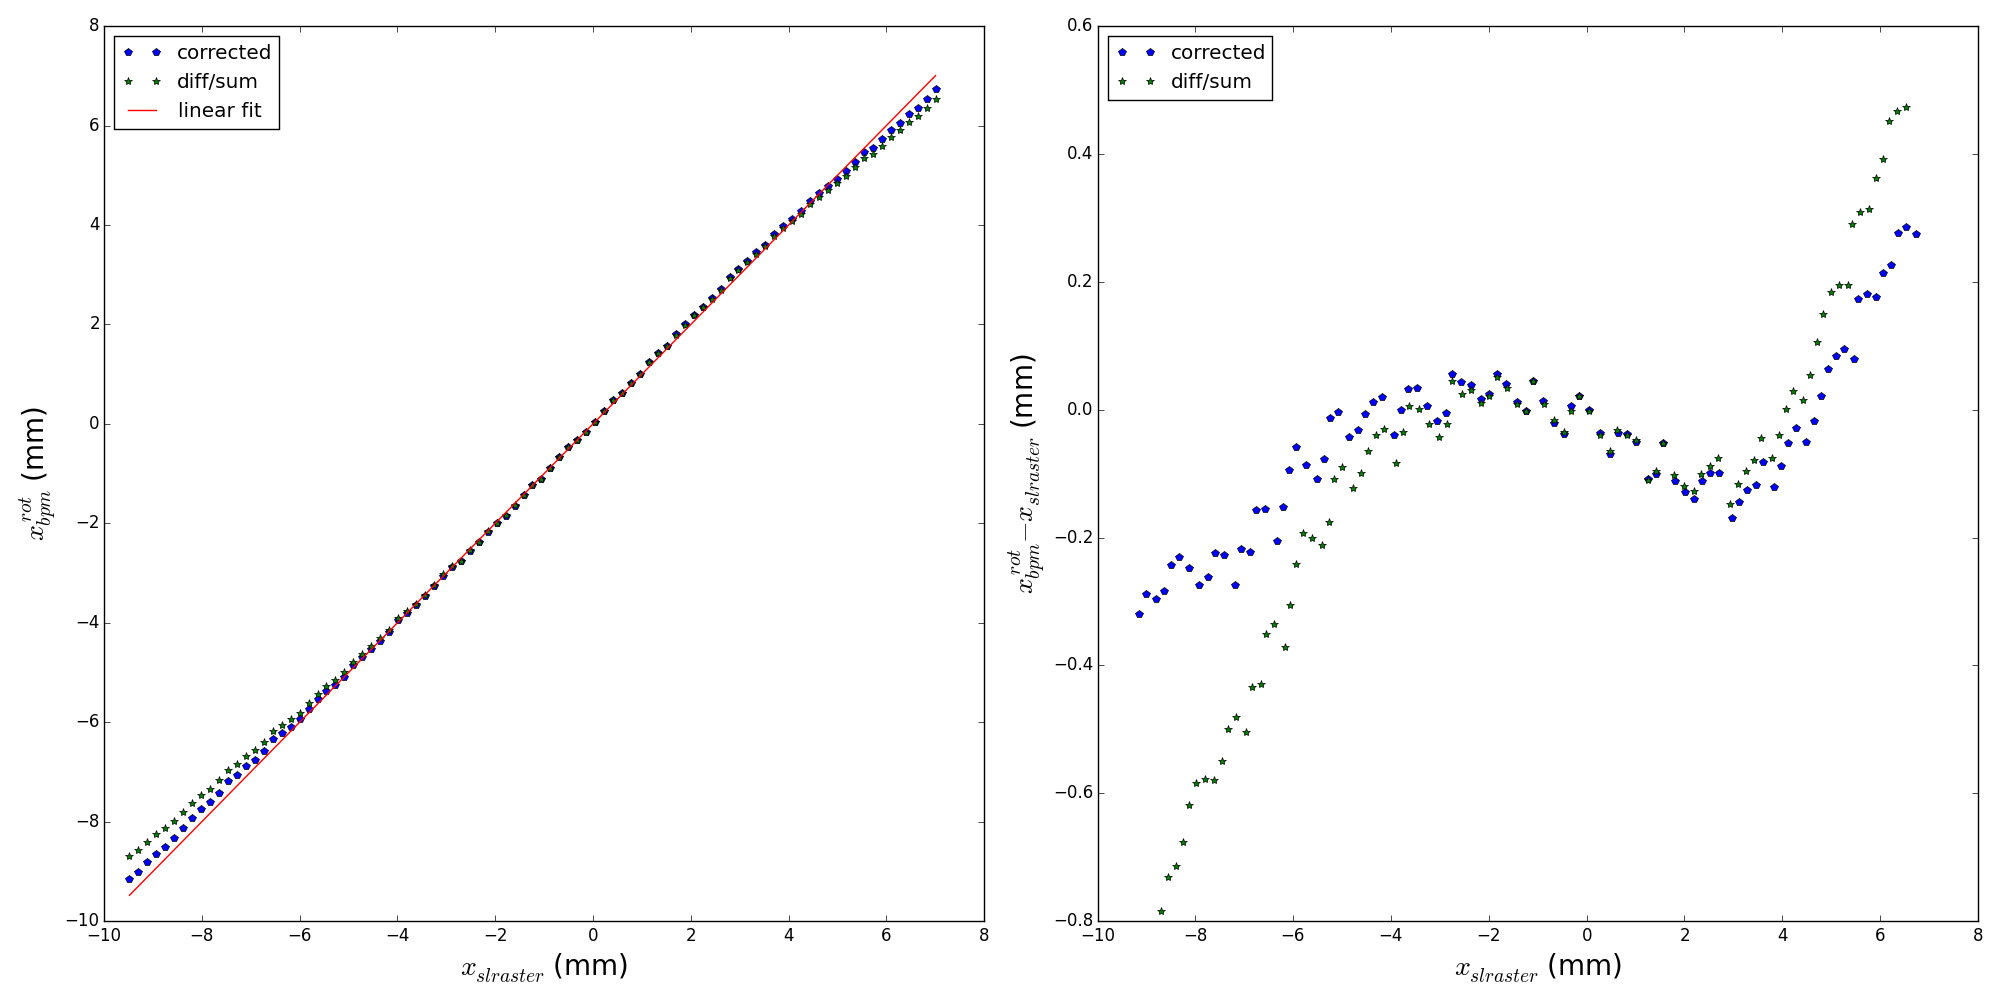
\includegraphics[width=0.9\linewidth]{raster_linear}
\par\end{centering}

\protect\caption{\label{fig:Linearityraster}Linearity of the corrected equation compared
with the diff/sum equation. The blue pentagon markers are calculated
from the corrected equation, while the green star markers are calculated
from the diff/sum equation. The x axis $x_{raster}$ is the position
transferred from the raster magnet current. The y axis in the left
side is the position calculated from the BPM in the rotated coordinate
system. The y axis in the right side is the absolute difference between
the position calculated from BPM and the position transferred from
the raster magnet current.}


\end{figure}
 The handling of the BPM information only used for the center beam
position (discussed in chapter \ref{sub:Det-ebe-pos}) also reduced
this non-linearity effect.

The final information recorded in the data-stream was designed to
have a linear response with the raw signal in the 50-100nA current
range. The $\phi_{i}$ in equation (\ref{eq:xb=00003D000026xy}) can
be rewritten as:

\begin{equation}
\phi_{i}=a_{i}(A_{i}-A_{i\_ped}+b_{i}),\label{eq:phivsA}
\end{equation}
where $A_{i}$ and $A_{i\_ped}$ are the recorded ADC value and pedestal
value, and $a_{i}$ and $b_{i}$ are the slope and intercept of the
relationship between $\phi_{i}$ and $A_{i}-A_{i\_ped}$. Equation
(\ref{eq:litexyb=00003D000026xy}) can be rewritten as:

\begin{eqnarray}
x_{d} & = & \frac{(A_{x+}-A_{x+\_ped}+b_{x+})-h_{x}(A_{x-}-A_{x-\_ped}+b_{x-})}{(A_{x+}-A_{x+\_ped}+b_{x+})+h_{x}(A_{x-}-A_{x-\_ped}+b_{x-})},\label{eq:xbfAb}\\
y_{d} & = & \frac{(A_{y+}-A_{y+\_ped}+b_{y+})-h_{y}(A_{y-}-A_{y-\_ped}+b_{y-})}{(A_{y+}-A_{y+\_ped}+b_{y+})+h_{y}(A_{y-}-A_{y-\_ped}+b_{y-})},\label{eq:ybfAb}
\end{eqnarray}
where $h_{x}$ = $a_{x-}/a_{x+}$, and is related to the ratio of
the signals for the $x_{+}$ and $x_{-}$ antennas and the gain settings
of the two channels. Similarly, $h_{y}=a_{y-}/a_{y+}$.

Combining the equation (\ref{eq:phivsA}) and (\ref{eq:antenna_signal}),
the calibration constant $b_{i}$ was obtained by taking the linear
fit between the ADC values of BPM and the beam current with a group
of runs with the same beam position but different values of beam current:
$I\propto(A_{i}-A_{i\_ped}+b_{i})$. 
\begin{figure}[tbph]
\begin{centering}
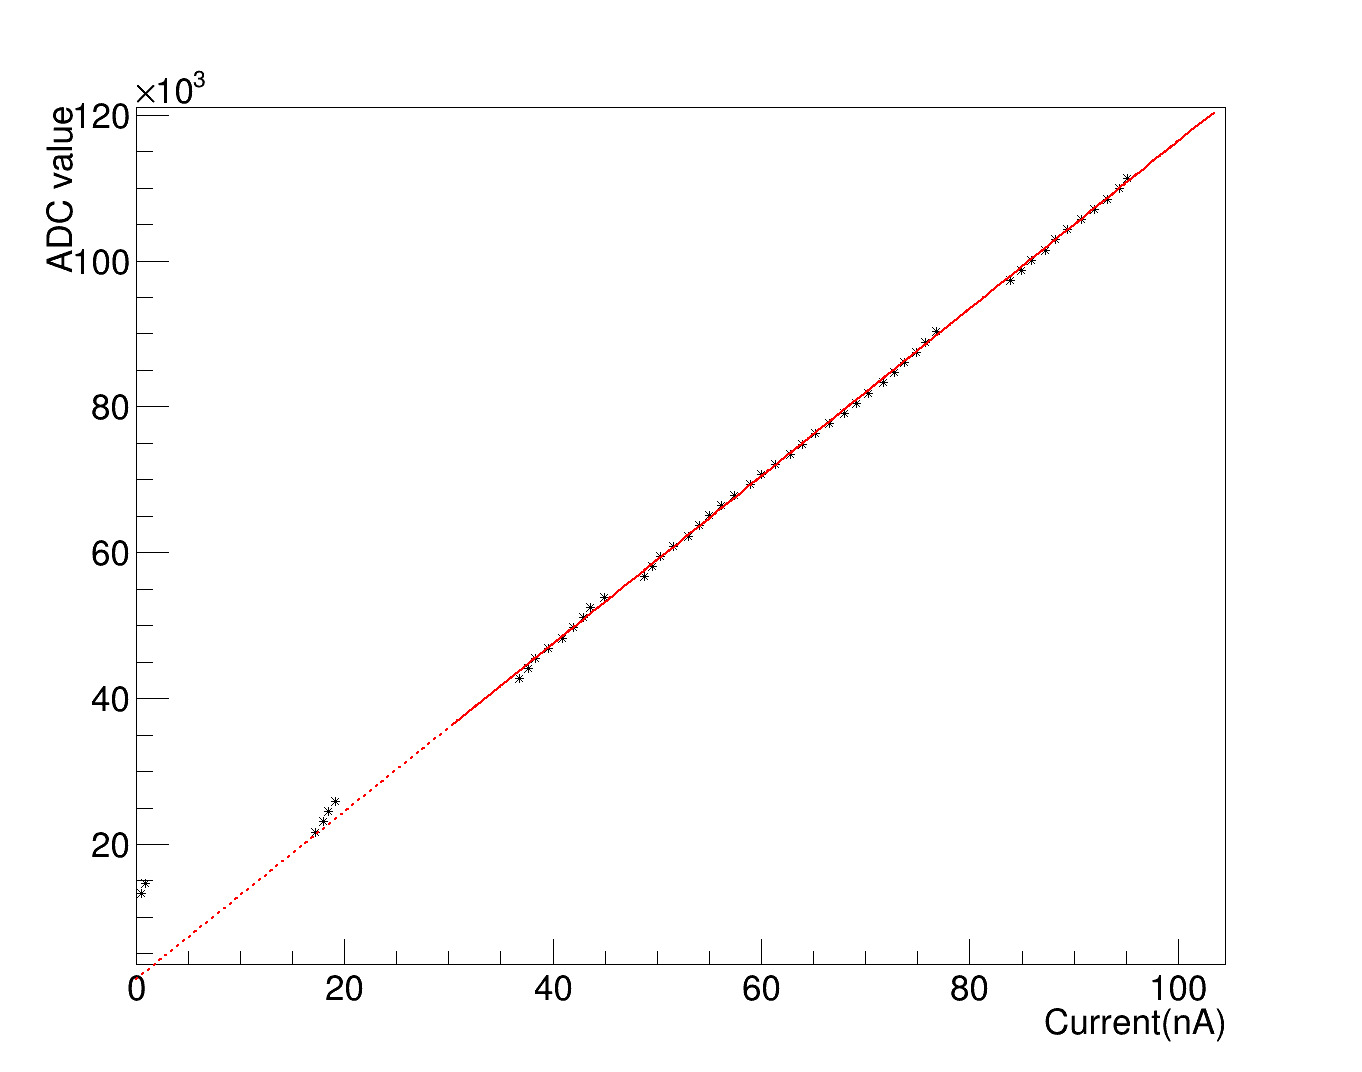
\includegraphics[width=0.5\linewidth]{currvspos} 
\par\end{centering}

\protect\caption{\label{fig:BPM-raw-signalVScurrent}ADC value of BPM raw signal ($A-A_{ped}$)
V.S. current}
\end{figure}
 Figure \ref{fig:BPM-raw-signalVScurrent} shows the $A_{i}-A_{i\_ped}$
versus the beam current. It can be seen that the ADC values were linear
with beam current in the considering current range of 50-100 nA. The
intercept from the linear fit of Fig.\ref{fig:BPM-raw-signalVScurrent}
is the value $b_{i}$. 

Combining a group of the harp scan data with a group of the BPM data,
the position determined from the harps was then used to calibrate
the $x$ and $y$ position calculated in equation (\ref{eq:realxy})
using the following equations:

\begin{eqnarray}
x_{harp}^{bpm} & = & c_{0}+c_{1}x+c_{2}y,\nonumber \\
y_{harp}^{bpm} & = & c_{0}'+c_{1}'x+c_{2}'y,\label{eq:harpvsxy}
\end{eqnarray}
where $x_{harp}^{bpm}$, $y_{harp}^{bpm}$ were projected from $x_{harp}$
and $y_{harp}$ in equation \ref{eq:harp}, $c_{0},c_{1},c_{2}$ and
$c_{0}',c_{1}',c_{2}'$ are the calibration constants, which from
a fit to the bpm data with the harp scan data, as an example shown
in Fig. \ref{fig:Harpscan}. 
\begin{figure}[tbph]
\begin{centering}
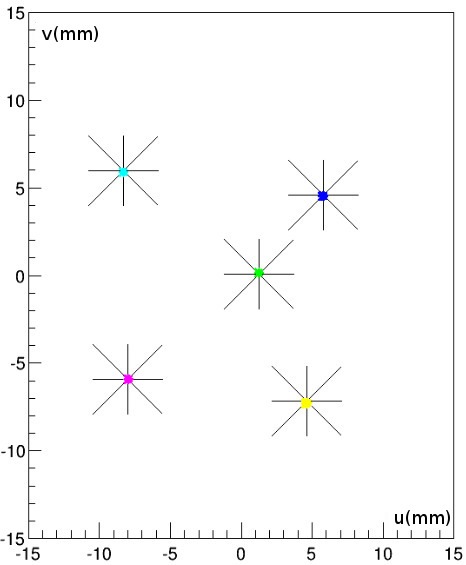
\includegraphics[width=0.4\linewidth]{harpscan}
\par\end{centering}

\protect\caption{\label{fig:Harpscan}Harp scan data combined with DAQ data, the asterisk
is the harp scan data, while the dot is the DAQ data after applying
the calibration constants. }
\end{figure}
 The asterisks in Fig. \ref{fig:Harpscan} represent the beam positions
$x_{harp}^{bpm}$ and $y_{harp}^{bpm}$ in the local coordinate of
the BPM calculated with the harp scan data, and the dots at the center
of the asterisks are the BPM data from the ADC after calibration.
Figure \ref{fig:Harpscan}(b) is the beam distribution recorded in
the ADC of the BPM with the slow raster on after applying the calibration
constants.

In order to reduce the noise and improve the resolution during data
analysis, a software filter was applied. Since the 18 bit ADC was
triggered by the helicity signal with a fixed frequency, it could
be regarded as a sampling ADC. 
\begin{figure}[tbph]
\begin{centering}
\subfloat[Normal run with beam]{\protect\begin{centering}
\protect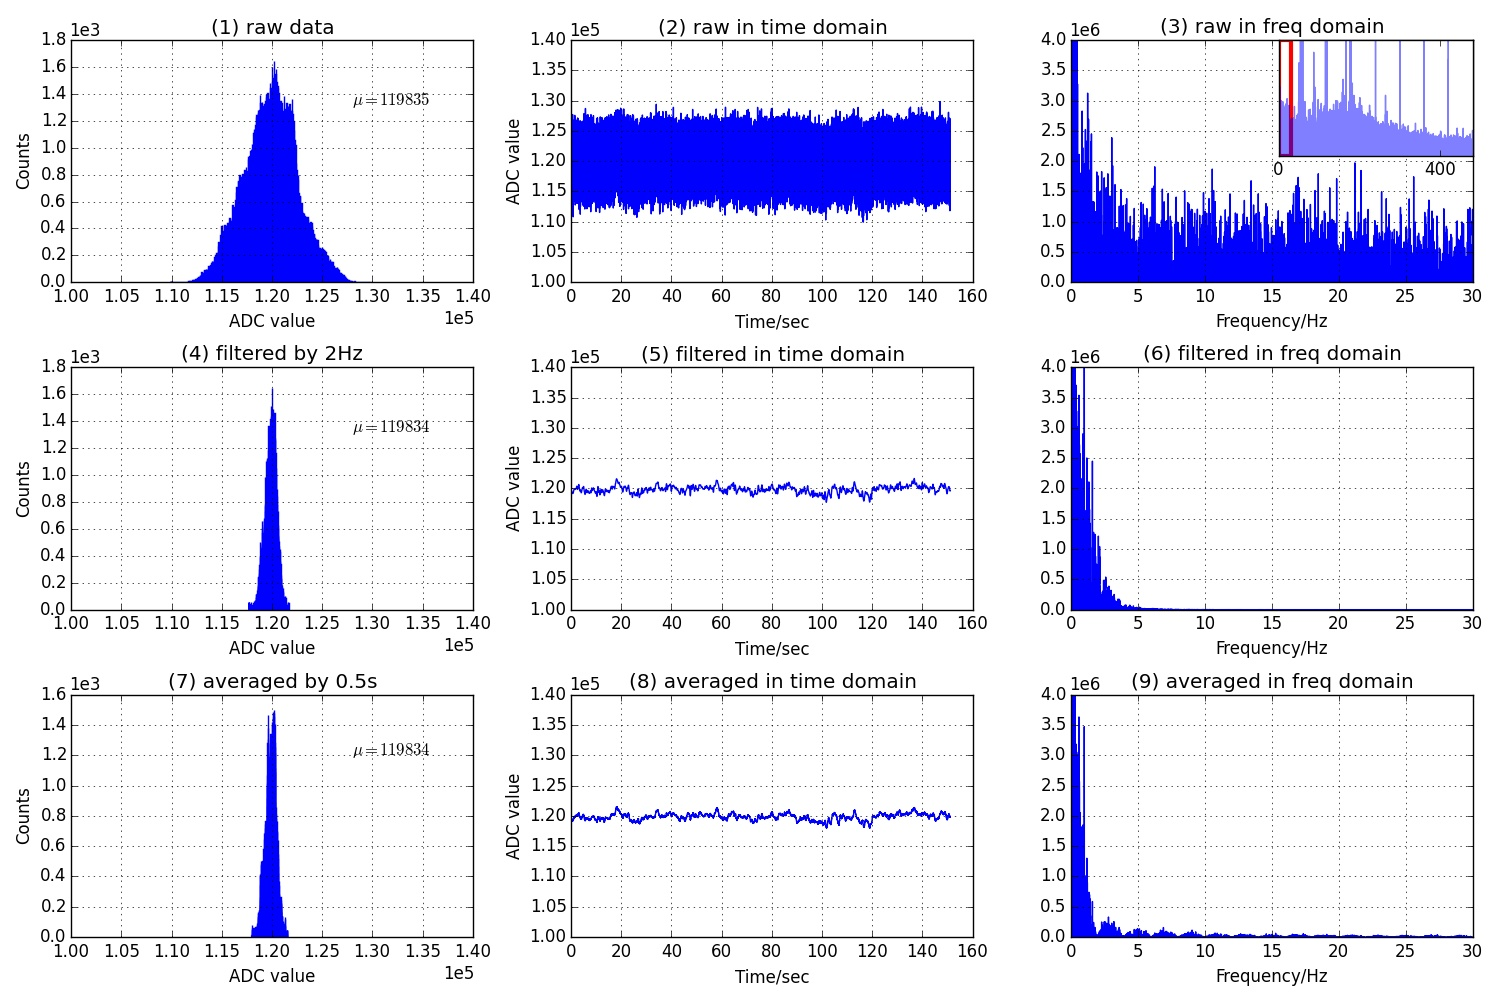
\includegraphics[width=0.9\columnwidth]{fft_signal}\protect
\par\end{centering}



}
\par\end{centering}

\begin{centering}
\subfloat[Pedestal run without beam]{\protect\begin{centering}
\protect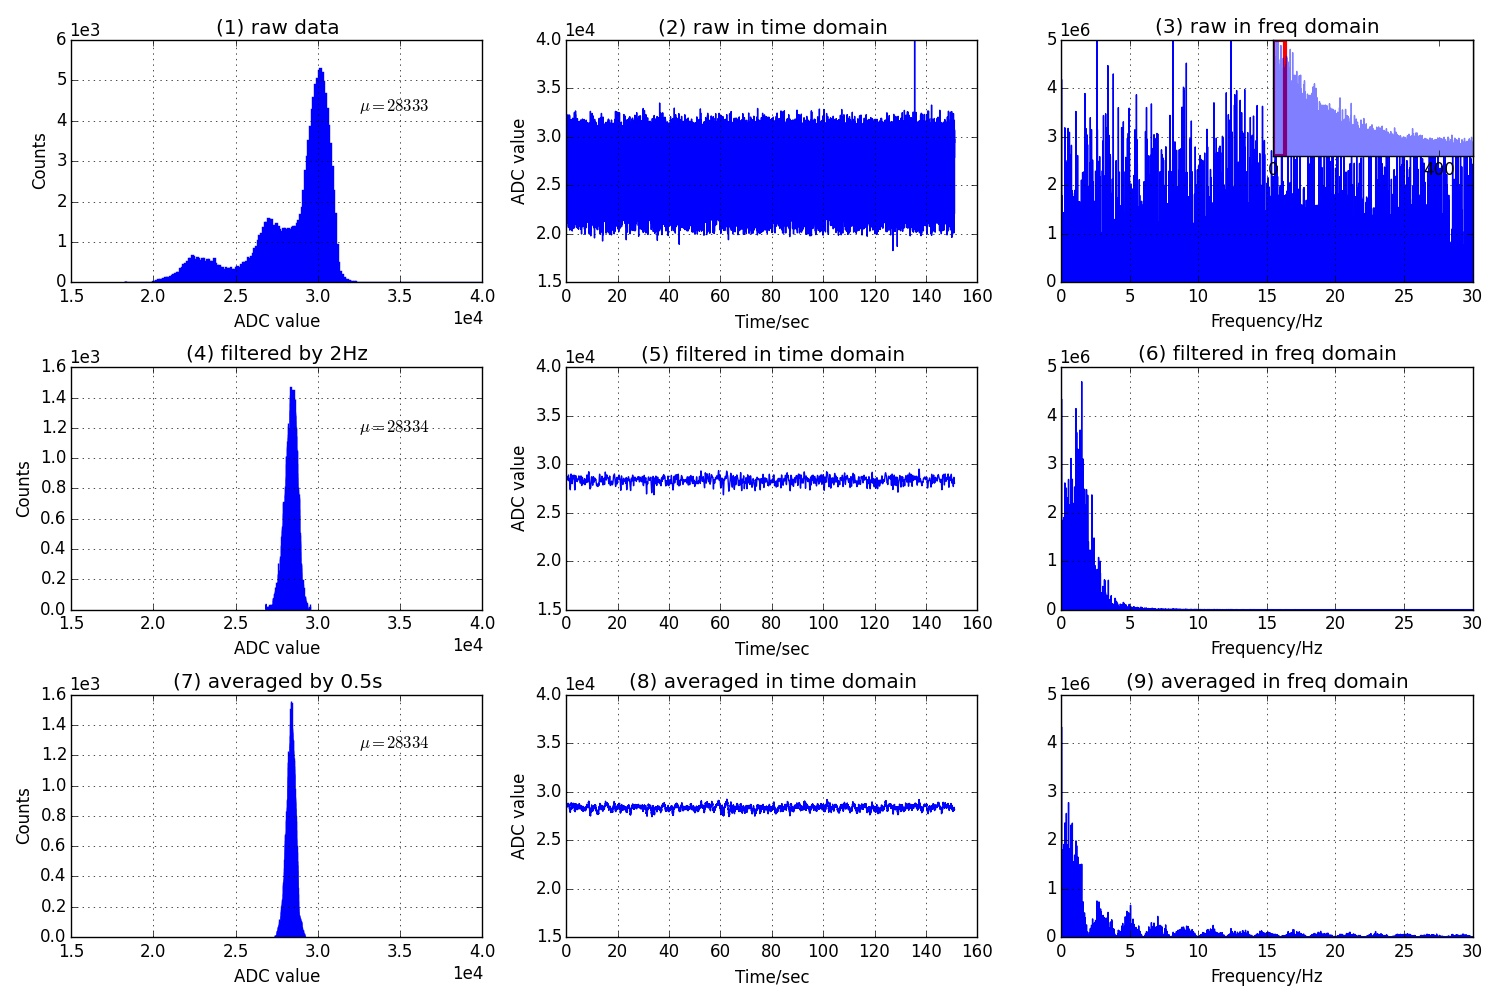
\includegraphics[width=0.9\columnwidth]{fft_pedestal}\protect
\par\end{centering}



}
\par\end{centering}

\protect\caption{\label{fig:2Hz-filter-added}Software filter applied to BPM signal.
(a) is the signal with beam, (b) is the pedestal signal without beam.
(1,2,3) in (a,b) are the raw signal without applying the filter, (4,5,6)
are applied a 2Hz finite-impulse-response filter with 4th order. (7,8,9)
are averaged with 0.5 s. (1,4,7) are the signal's 1-D histogram, (2,5,8)
are the signal in time domain, (3,6,9) are in frequency domain. Note
all of the plots in (a) is for a single signal, same as in (b).}
\end{figure}
 Fig.\ref{fig:2Hz-filter-added} shows the signal dealt with a 2 Hz
low pass filter. By sacrificing the high frequency signal, higher
resolution was gotten. The bottom 3 plots in Fig. \ref{fig:2Hz-filter-added}
(a,b) are the averaged signal for comparing with the filtered signal.
The average procedure also sacrificed the high frequency part of the
signal, which lead to the same result as the filter. The filter also
erases the beam displacement caused by the rasters, which is necessary
to extract the position of the beam center.


\subsection{Beam position reconstruction at the target\label{sub:Beam-position-reconstruction}}

It is easy to transport the position from the BPMs to the target by
using a linear transportation method for the straight through setting.
For the settings with a transverse magnetic field at the target, the
linear transportation method can not be used since the beam is bent
near the target. A simulation package was constructed to simulate
the behavior of the beam. Polynomial curve fittings were used for
simulated data to generate the transport functions in order to transport
the beam from the two BPMs to the target (Fig.\ref{fig:Transporting-beam-position}).
\begin{figure}[tbph]
\begin{centering}
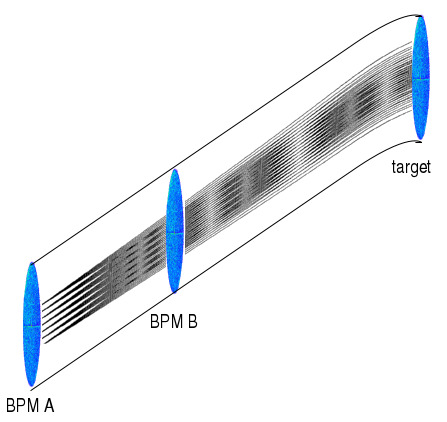
\includegraphics[width=0.4\linewidth]{rastersize_target1} 
\par\end{centering}

\protect\caption{\label{fig:Transporting-beam-position}Transporting beam position
from BPM to target with transverse target magnet field}
\end{figure}


A target magnet field map \citep{winestosca} was generated from the
TOSCA model. To test the accuracy of the TOSCA model, the target magnet
field was measured before the experiment \citep{jiefieldmap,chaofieldmap}.
The generated field map was used in the simulation. An event generator
generated thousands of electrons with different initial positions
and angles, with the energy of the electrons set to the same values
as in the experiment. The Runge-Kutta method\footnote{http://en.wikipedia.org/wiki/Runge\textendash Kutta\_methods}
with 0.02 mm step length was used to generate the trajectories from
BPM A to the target by using the field map. The positions at BPM A,
BPM B and the position and angle at the target were extracted from
the simulated trajectory.

Data extracted from the simulation was used as input to a fitting
program that determined the best-fit polynomial. In total, 24 different
fits were taken for 4 different target positions and 6 configurations
with different target magnetic field and beam energy settings. The
validity of the transport functions was explored in the simulation
using a new set of random trajectories generated in the same manner
as those used in the fitting. The deviation between the fitted transport
function and the simulation was less than 0.1\%.

The transport functions were only used to transport the beam center
position from the two BPMs to the target by applying the 2 Hz filter,
which filtered out the fast raster and slow raster motion to keep
only the beam center position. The transported position were expressed
as $X_{center}$ and $X_{center}$.


\subsection{\label{sub:Det-ebe-pos}Determining the beam position event-by-event}

The readout of the magnet current for the two rasters was connected
to a series of ADCs. Two scintillator planes in the HRS form a DAQ
trigger. This pulse signal triggered the ADC to record the raster
magnet current for each event. The information from the rasters and
the BPMs was combined to provide the beam position event-by-event.
The position at the target was determined as:

\begin{eqnarray}
X & = & X_{center}+X_{fstraster}+X_{slraster},\nonumber \\
Y & = & Y_{center}+Y_{fstraster}+Y_{slraster},\label{eq:total_pos}
\end{eqnarray}
where $X_{fstraster}$, $Y_{fstraster}$ and $X_{slraster}$, $Y_{slraster}$
were the position displaced by the fast raster and slow raster, respectively,
which were converted from the current values of the two raster magnets.
The calibration of the conversion factors between the magnet current
of the rasters and the displaced position will be discussed in the
next subsection. An example of reconstructed beam position is shown
in Fig. \ref{fig:Reconstructed-beam-position}.
\begin{figure}
\begin{centering}
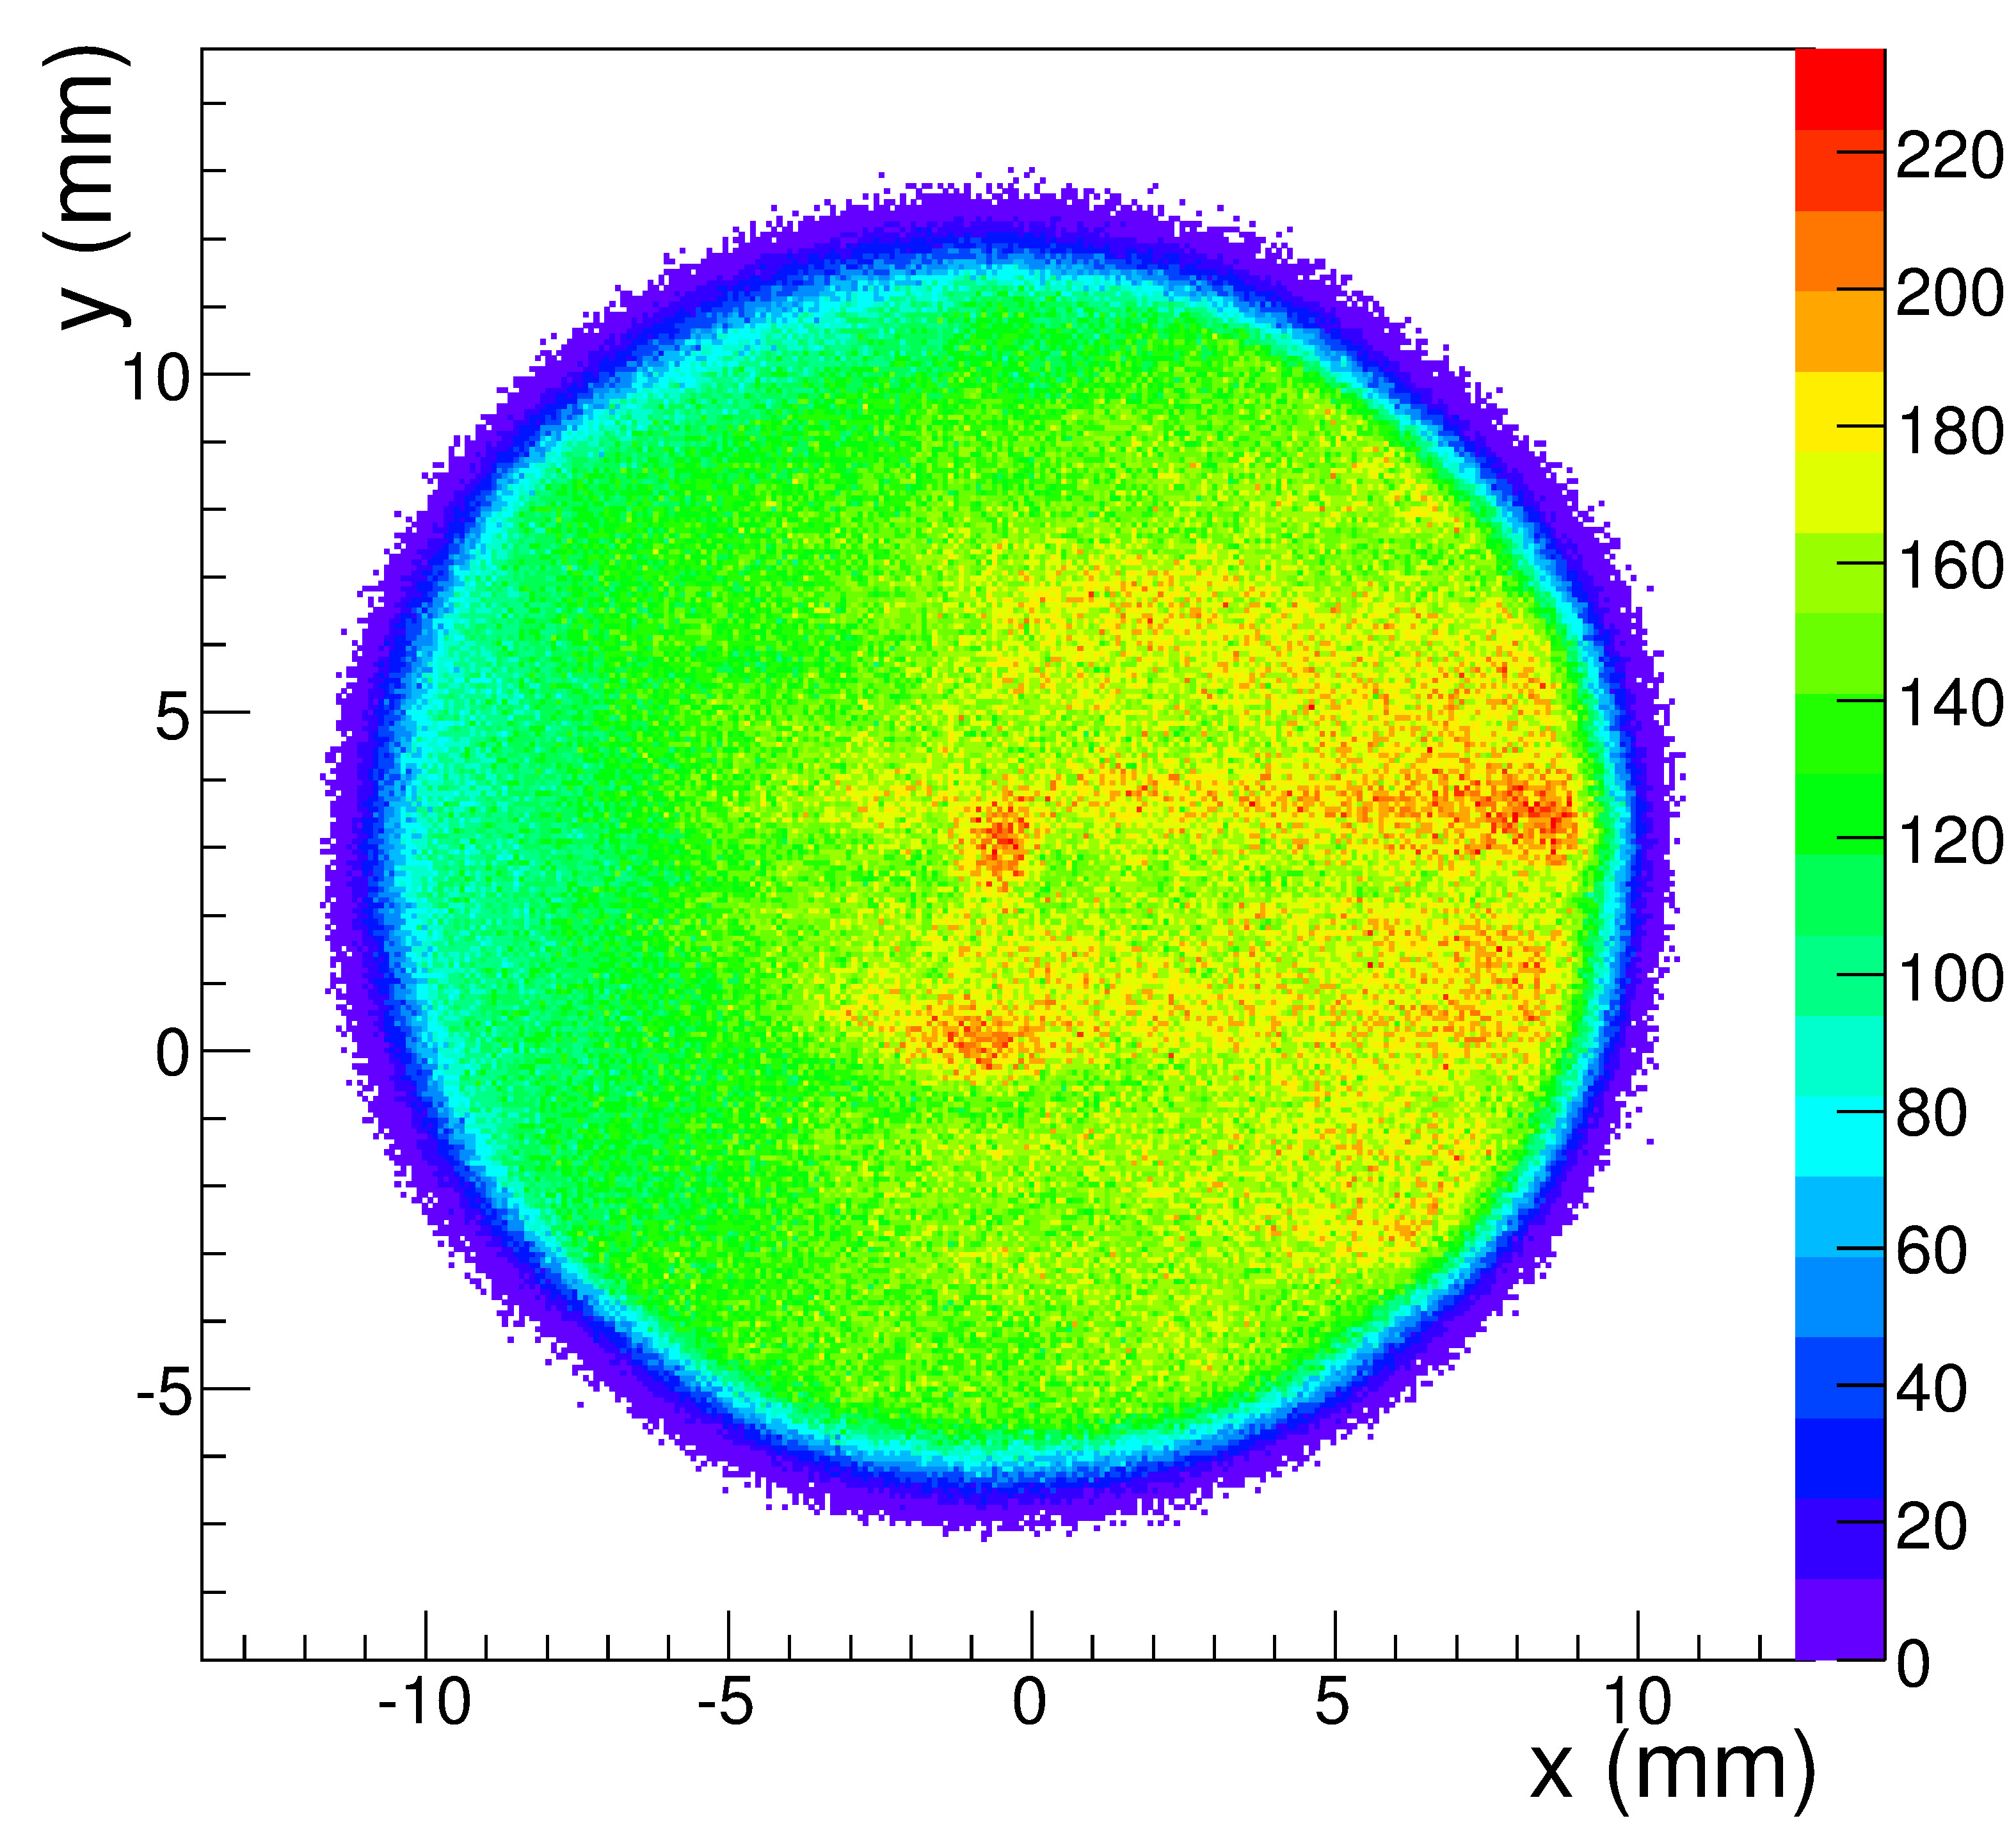
\includegraphics[width=0.6\columnwidth]{reconed}
\par\end{centering}

\protect\caption{\label{fig:Reconstructed-beam-position}Reconstructed beam position
at the target}


\end{figure}



\subsubsection{Conversion factor for the slow raster}

Two methods were used to calibrate the conversion factor for the slow
raster. The first method used the calibrated BPM information, i.e.,
comparing the raster magnet current with the beam shape shown in the
ADC of the BPMs. Several calibrations were taken during different
run periods at a beam current of 100nA using different values of the
raster magnet current, as shown in Fig.\ref{fig:Slow-raster-size}(a).
\begin{figure}[tbph]
\begin{centering}
\subfloat[\label{fig:slow-raster-run_different_size}ADC value of slow raster,
with the raster current changing]{\protect\begin{centering}
\protect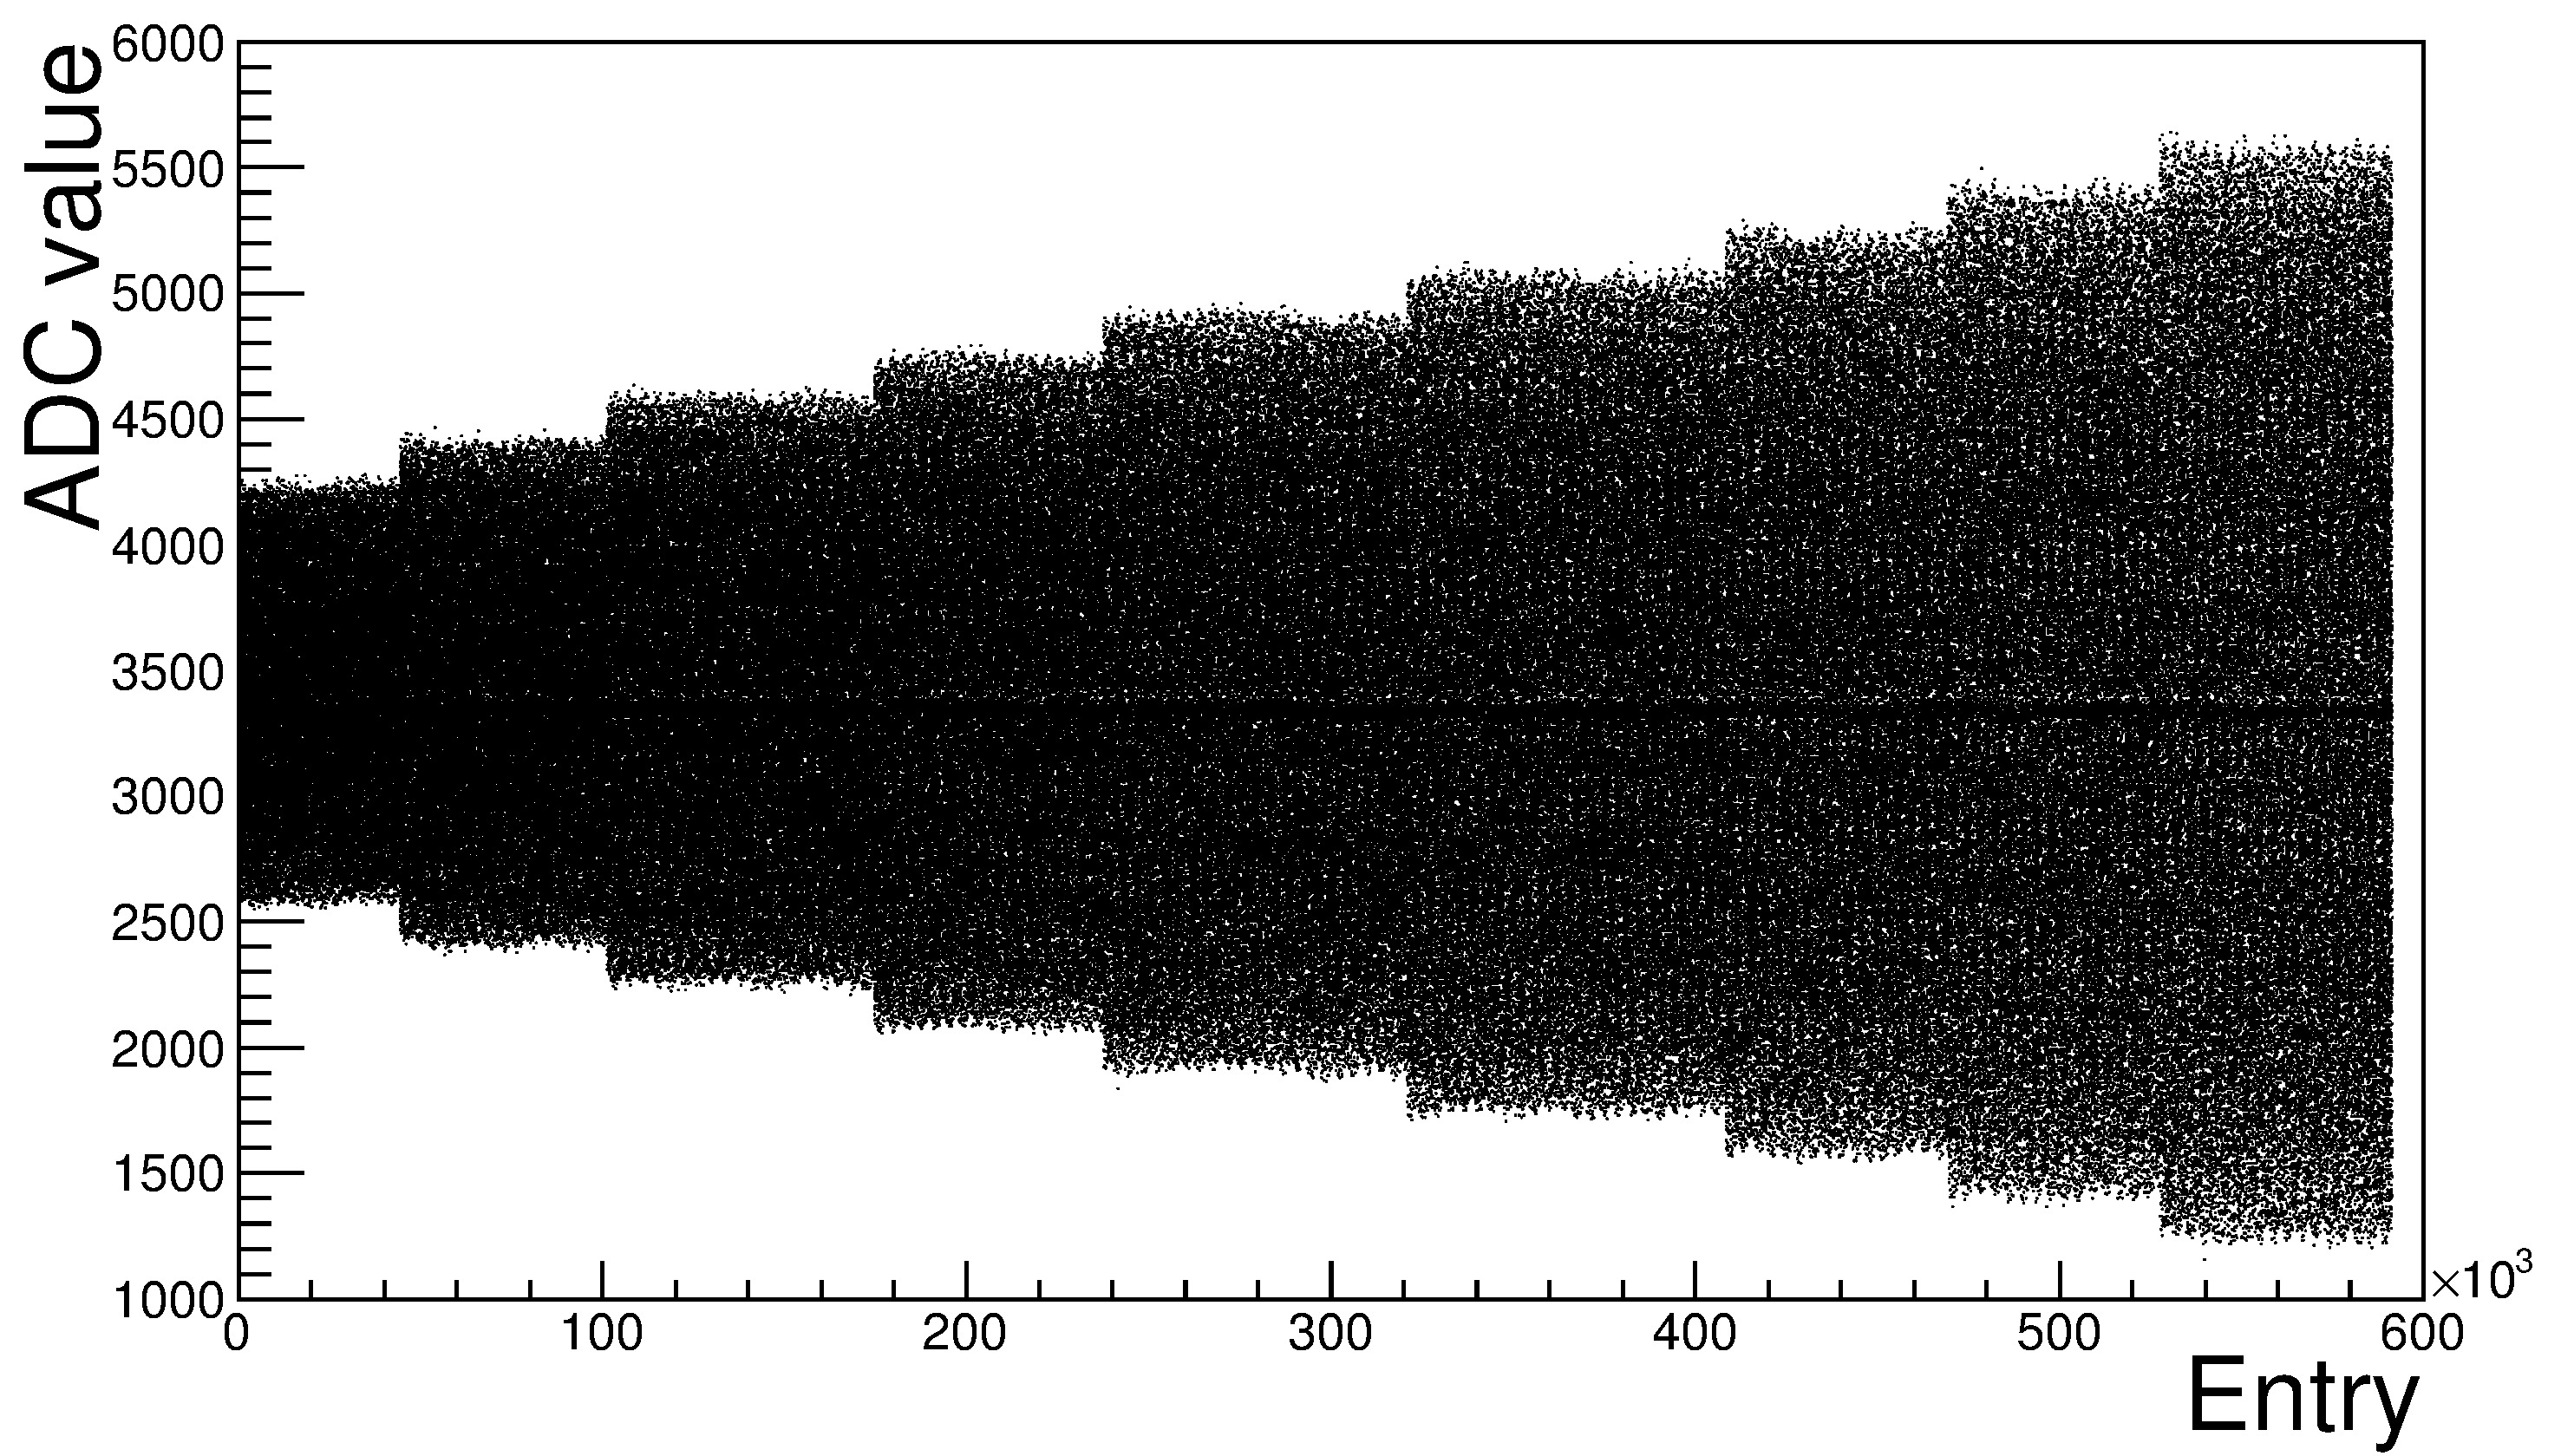
\includegraphics[width=0.33\linewidth]{raster_size_calib1}\protect
\par\end{centering}

}$\quad$\subfloat[\label{fig:slow-raster-oval-fit}Elliptical fit for the spread of
magnet current of slow raster]{\protect\begin{centering}
\protect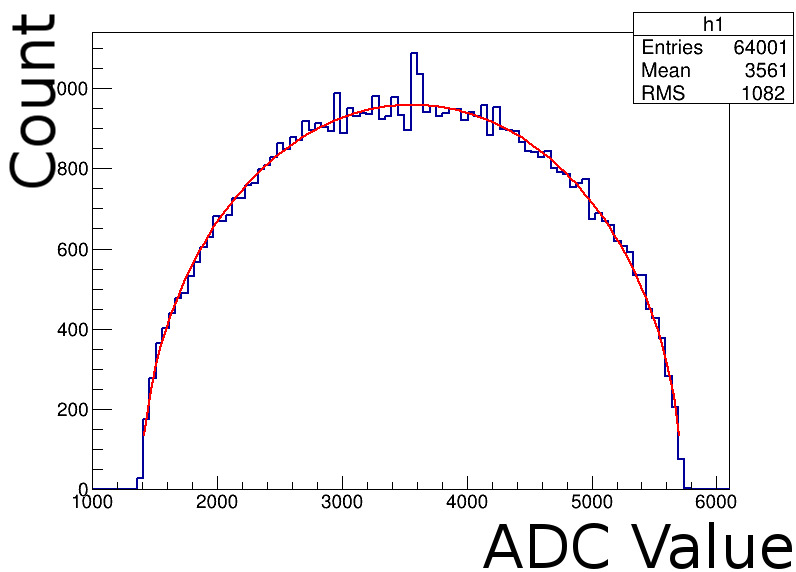
\includegraphics[width=0.28\linewidth]{slow_raster_oval_fit}\protect
\par\end{centering}

}$\quad$\subfloat[\label{fig:slow-raster-size_b}Linear fit between the raster current
and the range of beam distribution]{\protect\begin{centering}
\protect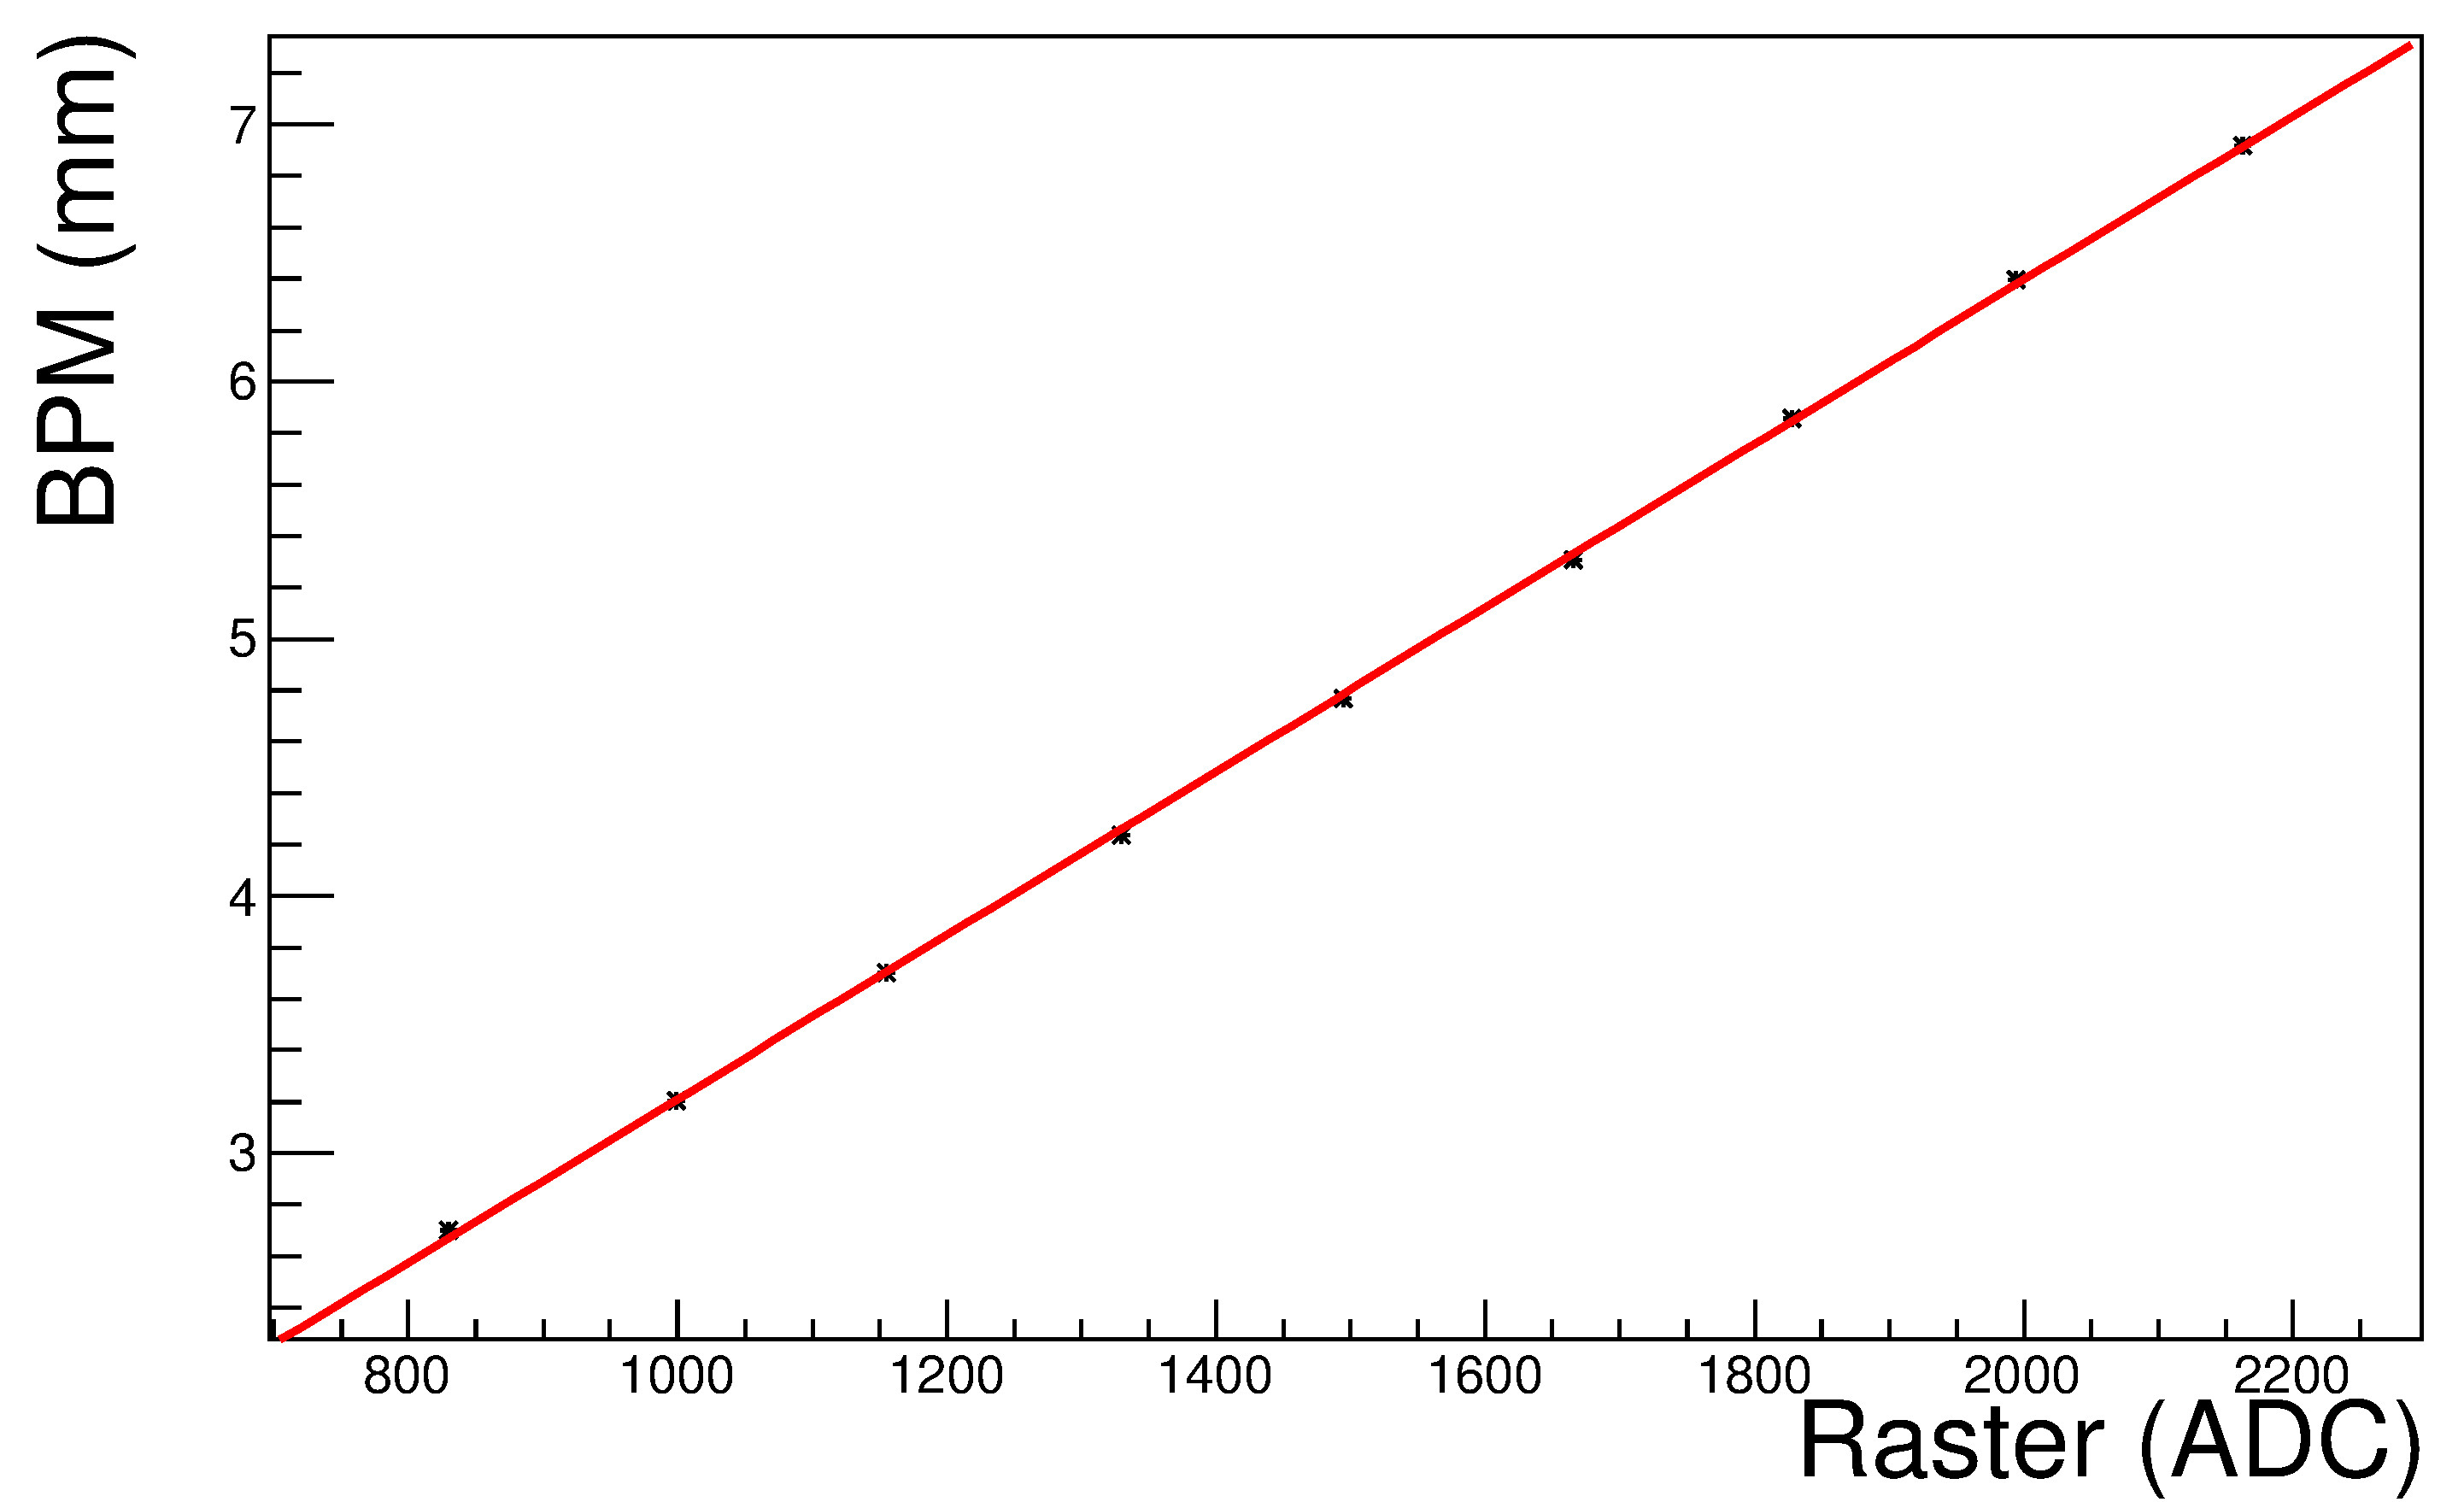
\includegraphics[width=0.3\linewidth]{raster_size_calib2}\protect
\par\end{centering}

}
\par\end{centering}

\protect\caption{\label{fig:Slow-raster-size}Converting the raster current to beam
position shift}
\end{figure}


The range of the beam distribution at the target was calculated from
the ranges at the two BPMs without applying the filter, using the
transport functions fitted previously. The range of the beam distribution
at the two BPMs and the amplitude of the raster current was calculated
from an elliptical fit, an example is shown in Fig.\ref{fig:Slow-raster-size}(b).
Figure \ref{fig:Slow-raster-size}(c) shows a linear fit between the
raster current and the range of the beam distribution at the target.
The x axis in Fig.\ref{fig:Slow-raster-size}(c) is the magnet current
of the raster, and the y axis is the range of the beam distribution
obtained from the BPMs.

The second method for calibrating the conversion factor used a target
called ``carbon hole'' as shown in Fig.\ref{fig:Carbon-hole}(a).
\begin{figure}[tbph]
\begin{centering}
\subfloat[Location for carbon hole target in target insert]{\protect\begin{centering}
\protect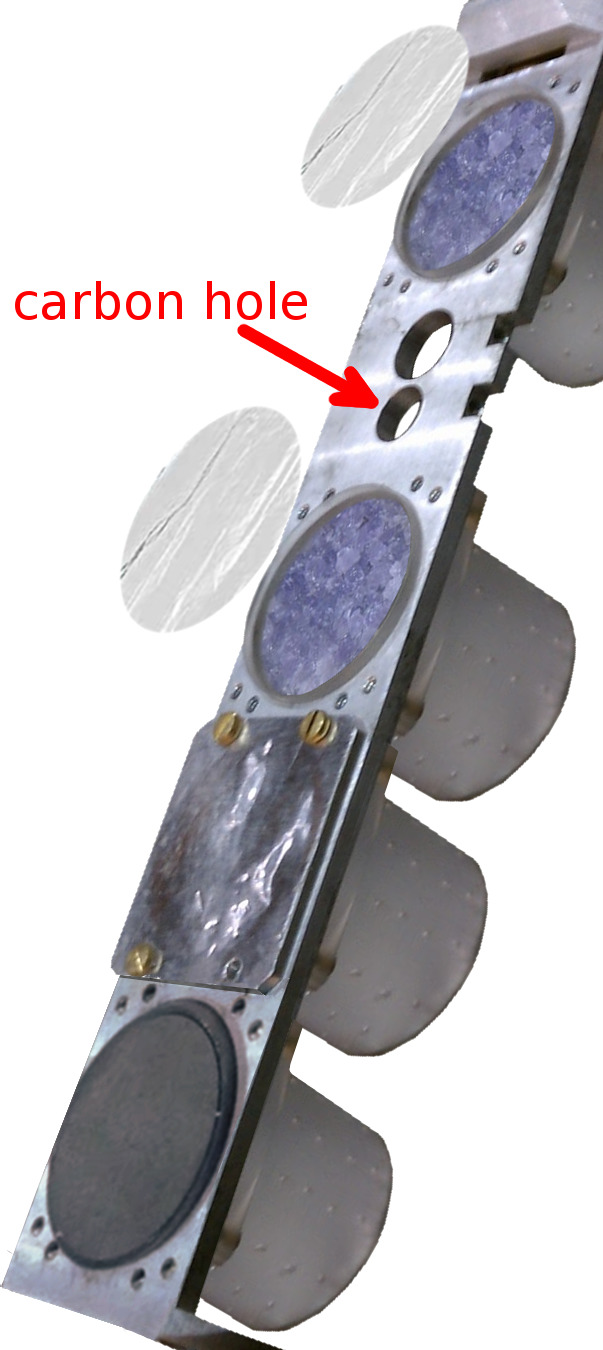
\includegraphics[width=0.23\linewidth]{enlarged-Target-insert}\protect
\par\end{centering}

}$\qquad$\subfloat[The shape of carbon hole in raster ADC, x and y axis are corresponding
to the currents on x magnet and y magnet of slow raster, respectively.]{\protect\begin{centering}
\protect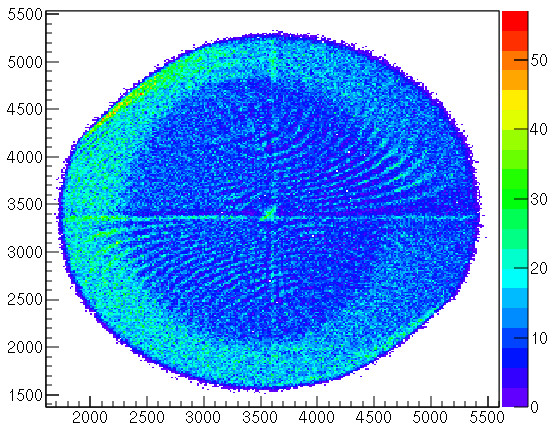
\includegraphics[width=0.58\textwidth]{carbon_hole}\protect
\par\end{centering}

}
\par\end{centering}

\protect\caption{\label{fig:Carbon-hole}Carbon hole method to calibrate raster}
\end{figure}


Scattered electrons were used as the trigger for recording the raster
magnet current. Since the density of the target frame was much higher
than that of the ``hole'', which was submerged in liquid helium,
the density of events triggered from the target frame was much higher
than that of the hole itself. Recorded values reveal a hole shape
as shown in Fig.\ref{fig:Carbon-hole}(b). The size of the carbon
hole was surveyed before the experiment, and a fit program was used
to extract the radius of the recorded hole shape for that raster current.
The conversion factor $F$ was then calculated as the ratio of the
size of the carbon hole $S_{hole}$ and the radius of the hole shape
$R_{hole}$ in the ADC:

\begin{equation}
F=\frac{S_{hole}}{2*R_{hole}}.\label{eq:convfactorhole}
\end{equation}



\subsubsection{Conversion factor for the fast raster}

The conversion for the fast raster was the same as for the slow raster.
The low pass filter for the BPM was set to a higher value than the
frequency of the fast raster to see the beam shape at the BPM formed
by the fast raster. For a higher frequency filter, a larger beam current
was needed to get a clear pattern. The beam current chosen for calibrating
the fast raster was near 300 nA, which was the safety limit for the
target. The beam shape formed by the fast raster is shown in Fig.\ref{fig:fastrasteratbpm}.
\begin{figure}[tbph]
\begin{centering}
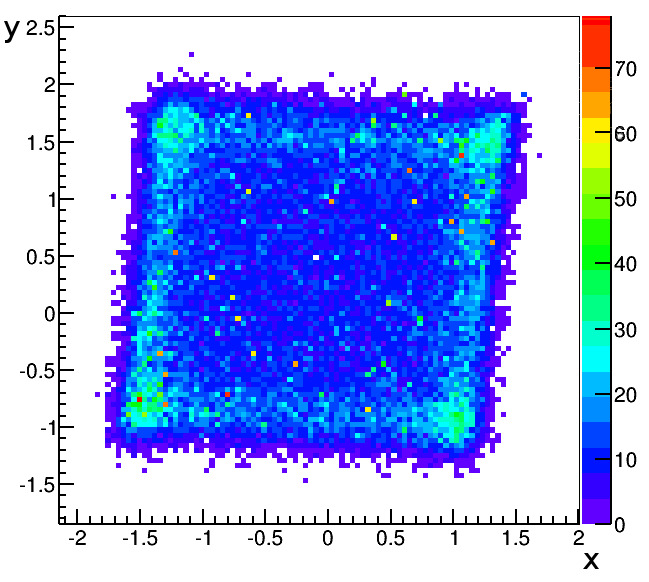
\includegraphics[width=0.5\columnwidth]{fastrasteratbpm} 
\par\end{centering}

\protect\caption{\label{fig:fastrasteratbpm}Beam shape formed by the fast raster at
the BPM A location, the unit is millimeter}
\end{figure}



\section{Uncertainty}

The uncertainty of the final beam position at the target for each
event contains several contributions: 
\begin{itemize}
\item The first part comes from the uncertainty of the calibration constant.
It includes the BPM resolution for the DAQ runs used for the calibration,
the uncertainty of the harp data corresponding to each calibration,
and the survey uncertainties for the BPMs and harps. It contributes
about 0.7 mm for the uncertainty of the position and 0.7 mrad for
the uncertainty of the angle. 
\item The uncertainty on the pedestal is the largest uncertainty for the
beam position measurement, contributing about 0.7$\sim$1.5 mm to
the uncertainty of the position and 0.7$\sim$1.5 mrad to the uncertainty
of the angle. 
\item The uncertainties from the BPM survey need to be included, since the
production data and the calibration data were taken at different beamline
settings when the equipment was moved. They contribute 0.5 mm to the
uncertainty of the position. 
\item The uncertainty from the magnetic field map of the target was considered
for the settings with the target magnet field. 
\item The uncertainties due to the size conversion of the rasters were also
included. 
\end{itemize}
The position uncertainty was magnified by a factor of 5 at the target
because of the short distance between the two BPMs. For example, in
the straight through setting, if the uncertainty at BPM A is 0.2 mm,
and at BPM B is 0.27 mm, the uncertainty at the target is 1.1 mm for
position and 1.3 mrad for angle. The uncertainty for the position
at the target was around 1$\sim$2 mm, while the uncertainty for the
angle was 1$\sim$2 mrad.


\section{Summary}

JLab g2p experiment used a transversely polarized $NH_{3}$ target
for the first time in Hall A. It put a limit of below 100 nA on the
electron beam current and required a slow raster to spread beam to
a large area. Two chicane magnets were used to compensate the strong
transverse magnetic field. Beam-line equipment, including the BPMs,
harps and associated readout system, were upgraded to allow precision
measurements of the beam position at low current (50-100 nA). A software
filter was used to reduce noise in the BPMs. A corrected equation
was used to compensate the non-linearity caused by the diff/sum equation.
The harp data and the linear fit between the bpm signal and the beam
current were used to extract the calibration constant of the BPM.
To account for the strong target magnetic field effect, transport
functions were generated to transport the beam position from the BPMs
to the target. The beam position in the x-y plane and the angle at
the target location are extracted event-by-event by combining information
from the BPMs and the signals from the rasters. The performance of
the new devices (BPMs, harps and slow rasters) were presented along
with an analysis of systematic uncertainties.


\section*{Acknowledgments}

This work was supported by DOE contract DE-AC05-84ER40150 under which
the Southeastern Universities Research Association (SURA) operates
the Thomas Jefferson National Accelerator Facility, and by the National
Natural Science Foundation of China (11135002, 11275083), the Natural
Science Foundation of Anhui Education Committee (KJ2012B179).


\section*{Reference}

\bibliographystyle{elsarticle-num}
\bibliography{bpm_paper}

\end{document}
